% **************************************************
% Macro specifiche per il documento corrente
% **************************************************
% Nome
\newcommand{\docName}{Specifica tecnica}
% Nome file
\newcommand{\docFileName}{specifica\_tecnica.1.0.pdf}
% Versione
\newcommand{\docVers}{0.1}
% Data creazione
\newcommand{\creationDate}{2013-01-16}
% Data ultima modifica
\newcommand{\modificationDate}{2013-01-17}
% Stato in {Approvato, Non approvato}
\newcommand{\docState}{Non approvato}
% Uso in {Interno, Esterno}
\newcommand{\docUsage}{Interno}
% Destinatari da specificare come nome1\\ &nome2\\ ecc.
\newcommand{\docDistributionList}{Team SoftwareSynthesis}
% Redattori da specificare come nome1\\ &nome2\\ ecc.
\newcommand{\docAuthors}{}
% Approvato da
\newcommand{\approvedBy}{}
% Verificatori
\newcommand{\verifiedBy}{}
% Perscorso (relativo o assoluto) che punta alla directory contenente shared/
% come sua sottodirectory (per comodità chiamiamola 'doc root').
\newcommand{\docRoot}{..}
% definire se si vuole l'indice delle tabelle
\def\INDICETABELLE{false}
% definire se si vuole l'indice delle figure
\def\INDICEFIGURE{true}

% importa il preambolo condiviso da tutti i documenti
% shared/preamble.tex
%
% Questo documento contiene la parte del preambolo condivisa e viene pertanto
% richiamato nel 'master' di tutti i documenti di progetto.  Al suo interno
% contiene le inclusioni (e le configurazioni) di tutti i package richiesti per
% la compilazione dei documenti, le macro di carattere generale e la definizione
% degli stili di pagina.

\documentclass[a4paper,10pt,openright]{article}

% **************************************************
% Macro generiche
% **************************************************
\newcommand{\team}{Software Synthesis}                    % chi siamo
\newcommand{\email}{software.synthesis@gmail.com}         % e-mail
\newcommand{\caName}{}                                    % titolo capitolato
\newcommand{\caDescr}{}                                   % descrizione
\newcommand{\inglese}[1]{\textit{#1}}

% **************************************************
% Codifica e lingua dei documenti
% **************************************************
\usepackage[utf8x]{inputenc}                              % codifica caratteri dei documenti sorgenti
\usepackage[english,italian]{babel}                       % localizzazione ai fini di sillabazione e cross-references
\usepackage[T1]{fontenc}                                  % codifica font di output

% **************************************************
% Definizione geometria della pagina
% **************************************************
\usepackage[a4paper,head=4cm,top=4.5cm,bottom=3cm,left=3cm,right=3cm,bindingoffset=5mm]{geometry}

% *************************************************
% Intestazioni e piè di pagina personalizzati
% *************************************************
\usepackage{fancyhdr}
% stile normale
\fancypagestyle{normal}{
\fancyhead{}                                              % intestazione
\fancyhead[RE,RO]{
\begin{picture}(0,0)
  \put(-410,0){
\includegraphics[width=1.02\textwidth]{header_logo}}
  \put(-410,10){\sffamily\large\leftmark}
\end{picture}
\vspace{-4pt}
}
\renewcommand{\headrulewidth}{.4pt}                       % riga sotto l'intestazione
\cfoot{}                                                  % piè di pagina
\fancyfoot[RO,LE]{\sffamily
  pag.~\thepage{} di \pageref{LastPage}}                  % a dx nelle pag. dispari e a sx in quelle pari
\fancyfoot[RE,LO]{\sffamily\docFileName{} -- v.\docVers}
\renewcommand{\footrulewidth}{.4pt}                       % riga sopra il piè di pagina
}
% stile per gli indici
\fancypagestyle{toc}{
\fancyhead{}                                              % intestazione
\fancyhead[RE,RO]{
\begin{picture}(0,0)
  \put(-410,0){
\includegraphics[width=1.02\textwidth]{header_logo}}
\end{picture}
}
\renewcommand{\headrule}{}                                % nessuna riga sotto l'intestazione
\cfoot{}                                                  % piè di pagina
\fancyfoot[RO,LE]{\sffamily\thepage{}}                    % a dx nelle pag. dispari e a sx in quelle pari
\fancyfoot[RE,LO]{\sffamily\docFileName{} -- v.\docVers}
\renewcommand{\footrulewidth}{.4pt}                       % riga sopra il piè di pagina
}

\pagestyle{fancy}                                         % premetto: non so usare bene le marche:
\renewcommand{\sectionmark}[1]{\markboth{#1}{#1}}         % se qualcuno ha idee migliori si faccia avanti!

% **************************************************
% Tabelle
% **************************************************
\usepackage{tabularx}                                     % tabelle di larghezza fissa con una o più colonne variabili
\usepackage{multirow}                                     % colonne con colonne che si estendono per più righe
\usepackage{booktabs}                                     % per inserire l'ambiente table e le righe orizz. nelle tabelle
\usepackage{longtable}			                          % tabelle oltre i limiti di pagina

% **************************************************
% Cross-references e collegamenti ipertestuali
% **************************************************
\usepackage[hidelinks]{hyperref}
\hypersetup{%
  colorlinks=false, linktocpage=false, pdfborder={0,0,0}, pdfstartpage=3, pdfstartview=FitV,%
  urlcolor=Cyan, linkcolor=Cyan, citecolor=Black, %pagecolor=Black,%
  pdftitle={\docName}, pdfauthor={\team}, pdfsubject={}, pdfkeywords={},%
  pdfcreator={pdflatex}, pdfproducer={pdflatex with hyperref package}%
}

% **************************************************
% Immagini e grafica
% **************************************************
\usepackage{graphicx}                                     % supporto ad aspetti avanzati delle immagini
\graphicspath{{\docRoot/pics/}}                           % percorso contenente tutti i file immagini
\usepackage{color}                                        % permette di colorare facilmente il testo

% **************************************************
% Altri pacchetti opzionali
% **************************************************     
\usepackage{lastpage}                                     % per sapere il numero totale di pagine
\usepackage{lipsum}                                       % genera "dummy text" per prove di impaginazione
\usepackage{eurosym}                                      % per il simbolo dell'euro usare \EUR{x} dove x è l'importo


% Fine del preambolo e inizio del documento
\begin{document}

% Inclusione della prima pagina
% shared/firstpage.tex
%
% Questo documento definisce il contenuto della prima pagina, che si suppone
% essere uguale in tutti i documenti.  Oltre al logo e al titolo, la prima
% pagina contiene i metadati relativi al documento in cui viene inclusa.


% rimuove intestazioni e piè di pagina
\pagestyle{empty}

\begin{center}

% logo del gruppo

\includegraphics[width=1.5\textwidth]{logo}

\vspace{1in}

% titolo del documento
{\Huge\bfseries \docName}

\vspace{1in}

% tabella riepilogativa
\begin{tabularx}{.7\textwidth}{>{\bfseries\sffamily}l>{\sffamily}l}
\toprule
\multicolumn{2}{>{\sffamily}c}{Informazioni sul documento}\\
\midrule
Nome file:            & \docFileName\\
Versione:             & \docVers\\
Data creazione:       & \creationDate\\
Data ultima modifica: & \modificationDate\\
Stato:                & \docState\\
Uso:                  & \docUsage\\
Redattori:            & \docAuthors\\
Approvato da:         & \approvedBy\\
Verificatori:         & \verifiedBy\\
\bottomrule
\end{tabularx}

\end{center}

\newpage


%---------------------------RUOLI----------------------------
%FASE 1:
%Progettisti: TRES, STEFANO, SCHIVO;
%FASE 2:
%Progettisti: DIEGO, ELENA, RIZZI

%Verificatore: Andrea Meneghinello
%Responsabile finale TRES
%------------------------------------------------------------

% Storico delle modifiche
\section*{Storia delle modifiche}
\begin{center}
\begin{longtable}{lp{.32\textwidth}lll}
\toprule
Versione & Descrizione intervento & Membro & Ruolo & Data\\
\midrule % inserire qui il contenuto della tabella
0.2 & Stesura dell'introduzione ai design pattern. Stesura dell'introduzione ai tracciamenti. & Stefano Farronato & Progettista & 2013-01-17\\
0.1 & Creazione del documento e stesura della sezione ``Introduzione''. & Riccardo Tresoldi & Progettista & 2013-01-16\\
\bottomrule
\end{longtable}
\end{center}
\newpage

% inclusione dell'indice
% shared/toc.tex
%
% Questo file contiene le istruzioni che generano l'indice o gli indici del
% documento (utile nel caso in cui decidessimo di avere anche un indice delle
% tabelle e/o un indice delle figure).

\pagestyle{toc}
\pagenumbering{roman}

\tableofcontents

\newpage


% Alcuni aggiustamenti per le pagine
\pagenumbering{arabic}
\setcounter{page}{1}
\pagestyle{normal}

% Qui ha inizio il documento vero e proprio...
\newpage

\section{Introduzione}
\subsection{Scopo del prodotto}
\purpose

\subsection{Scopo del documento}
Il presente documento è stato redatto al fine di produrre le specifiche sulla progettazione ad alto livello, del prodotto \caName. A tal fine il documento presenterà:
\begin{itemize}
    \item una descrizione degli strumenti e dei framework su cui si basa l'architettura;
	\item un elenco con le specifiche dei design pattern utilizzati;
	\item l'architettura di alto livello del sistema;
	\item una descrizione dettagliata dei componenti rilevati in fase di progettazione indicando relativamente a ciascuno di essi il tipo, la funzione e l'obiettivo;
	\item i diagrammi UML per definire i flussi principali di controllo dell'applicativo;
	\item il tracciamento dei requisiti e dei componenti, negli schemi: requisiti-componenti e componenti-requisiti;
	\item il tracciamento di componenti e design pattern;
	\item il tracciamento di classi e componenti.
\end{itemize}

\subsection{Glossario}
\glossaryIntro

\clearpage
\section{Riferimenti}

\subsection{Normativi}
\begin{itemize}
\item[] \textit{piano\_di\_qualifica.2.0.pdf} allegato.
\item[] \textit{norme\_di\_progetto.2.0.pdf} allegato.
\item[] \textit{analisi\_dei\_requisiti.2.0.pdf} allegato
\end{itemize}

\subsection{Informativi}
\begin{itemize}
\item[] Capitolato d'appalto: \caName{}, v1.0, redatto e rilasciato dal proponente Zucchetti s.r.l. reperibile all'indirizzo \url{http://www.math.unipd.it/~tullio/IS-1/2012/Progetto/C1.pdf};
\item[] testo di consultazione: \textit{Software Engineering (8th edition) Ian Sommerville, Pearson Education | Addison Wesley};
\item[] manuale all'utilizzo dei design pattens: \textit{Design Patterns, Elementi per il riuso di software a oggetti -- (1/Ed. italiana) Eric Gamma, Richard Helm, Ralph Johnson, John Vlissides, Pearson Education};
\item[] manuale di basi di dati: \textit{Titolo: Sistemi di basi di dati-fondamenti} -- (6° edizione) Ramez Elmasri / Shamkant B. Navathe
\item[] \textit{glossario.1.0.pdf} allegato.
\end{itemize}
\clearpage

\section{Strumenti utilizzati}
\subsection{Java}
L'utilizzo del linguaggio Java è richiesto dal proponente solo per il lato server.

\subsubsection*{Vantaggi}
\begin{itemize}
\item[-] è un linguaggio predisposto nativamente alla gestione parallela di thread e questo applicato ad un server dà la possibilità di gestire parallelamente richieste da parte di più utenti allo stesso tempo;
\item[-] essendo un linguaggio orientato agli oggetti e fortemente tipizzato si presta all'applicazione di design pattern e alla costruzione di un'architettura robusta, fortemente modulare e al contempo flessibile, in accordo con i principi del paradigma di programmazione OO;
\item[-] permette la generazione automatica della documentazione con l'ausilio di JavaDoc;
\item[-] garantisce la portabilità del codice (a livello di bytecode), l'indipendenza dalla piattaforma fisica di esecuzione grazie alla JVM e l'integrazione nell'ambiente di esecuzione del proponente (TomCat).
\end{itemize}
\subsubsection*{Svantaggi}
\begin{itemize}
\item[-] potenziale lentezza causata dall'utilizzo della JVM e dal fatto di essere un linguaggio interpretato.
\end{itemize}

\subsection{Hibernate}
Hibernate è un framework Java utilizzato per facilitare l'utilizzo di un database da parte del server realizzando la mappatura fra oggetti intesi in senso OOP ed ennuple del modello relazionale (Object-Relational Mapping).

\subsubsection*{Vantaggi}
\begin{itemize}
\item[-] Hibernate permette di utilizzare le tabelle di un database relazionale come se fossero degli oggetti mappando il database su di opportune classi strutturate ad-hoc svincolando la gestione della persistenza dei dati dalla logica di business;
\item[-] con questo framework Java riesce a lavorare su un database rendendo trasparenti al programmatore le vere e proprie query e mostrando esclusivamente classi e metodi;
\item[-] essendo rilasciato sotto licenza LGPL può essere utilizzato senza restrizioni (copyleft) e vincoli di licenza delle opere derivate. 
\end{itemize}
\clearpage

\section{Design Pattern}
In questa sezione discuteremo i design pattern utilizzati nella progettazione dei componenti architetturali. Ogni design pattern sarà proposto con la seguente forma:
\begin{itemize}
	\item \textbf{Scopo}: verrà proposto lo scopo generico del pattern, al fine di evidenziare subito la sua utilità.
	\item \textbf{Diagramma esemplificativo}: si riporterà lo schema UML, rappresentante un implementazione generica del design pattern in esame.
	\item \textbf{Vantaggi derivanti}: si darà un elenco dei vantaggi apportati dall'utilizzo del pattern, in particolare sotto il profilo della manutenzione e del riuso del codice.
	\item \textbf{Componenti che lo implementano}: infine verranno elencati i componenti dell'architettura di sistema, che implementano il pattern descritto.
\end{itemize}

Per una visione d'insieme dei componenti utilizzati da un pattern, e dei pattern utilizzati da un componente, rimandiamo alle sottosezioni ``Tracciamenti Componenti-Design Pattern'' e ``Tracciamenti Design Pattern-Componenti'' della sezione ``Tracciamenti''.

\subsection{Composite}

\subsubsection{Scopo}
Il pattern Composite ha lo scopo di comporre oggetti in strutture ad albero al fine di rappresentare gerarchie parte-tutto e consentire ai \underline{client} di trattare oggetti singoli e composizioni in modo uniforme. Permette inoltre di gestire strutture dati gerarchicizzate con elementi ``foglie'' ed elementi ``contenitori'', l'ideale per la struttura ``gruppo'' e ``utente''.

\subsubsection{Diagramma esemplificativo}
\begin{figure}[h]
\centering
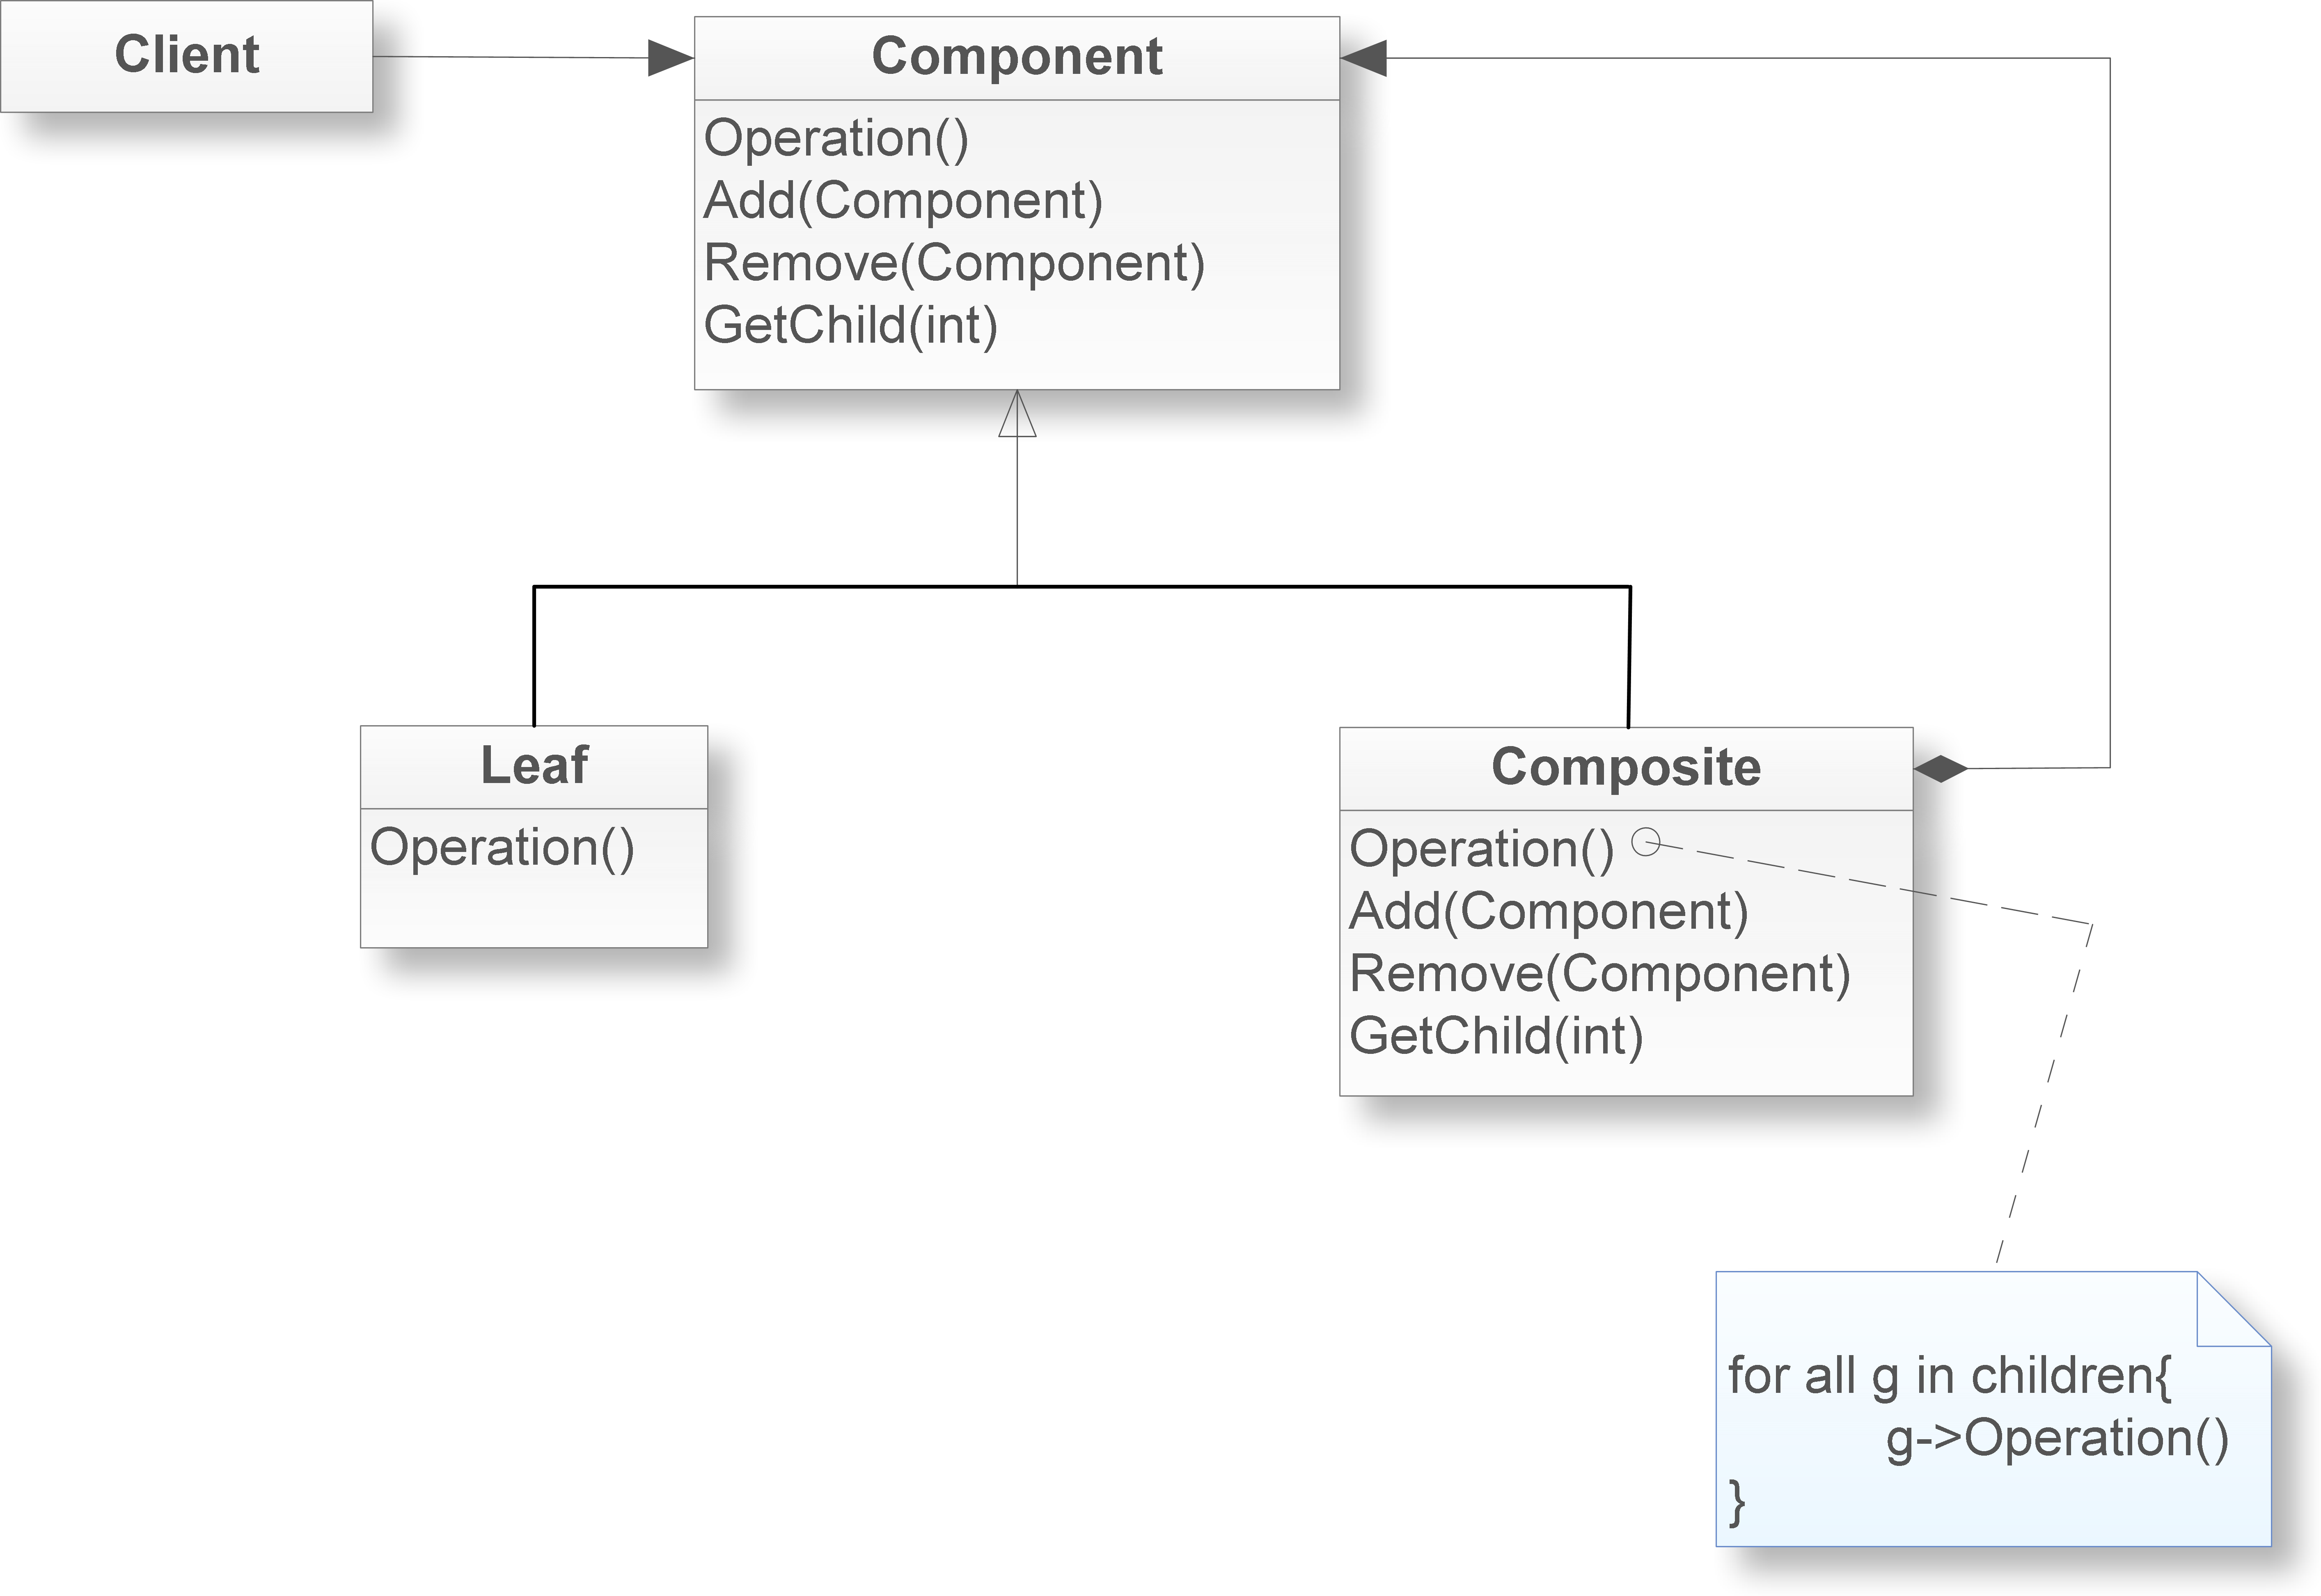
\includegraphics[width=.8\textwidth]{composite}
\caption{Diagramma ad alto livello del pattern Composite.}\label{fig:composite}
\end{figure}

\subsubsection{Componenti che lo implementano}
\begin{description}
\item{\bfseries\scshape Gestione della rubrica (lato server)}\\
Composite permette di trattare in maniera omogenea singoli oggetti e oggetti composti, come gli utenti e gruppi di utenti della rubrica. Inoltre, dal momento che rende più semplice l'aggiunta di componenti, permetterebbe in futuro l'integrazione di nuove tipologie di utenti senza la necessità di modificare la struttura preesistente.

Lo svantaggio principale che comporta l'uso di Composite è la mancanza di limiti nell'aggiunta di nuove tipologie di componenti. Per far fronte a questo rischio si è introdotta la classe \texttt{org.softwaresynthesis.mytalk.server.abook.AddressBook} che controlla l'accesso alla struttura dati corrispondente alla rubrica.
\end{description}

\subsection{Data Access Object (DAO)}

\subsubsection{Scopo}
Il pattern DAO ha lo scopo di disaccoppiare la logica di business dalla logica di accesso ai dati. Questo si ottiene spostando la logica di accesso ai dati dai componenti di business ad una classe DAO rendendo i componenti che implementano la logica di business indipendenti dalla natura del dispositivo di persistenza. Questo approccio garantisce che un eventuale cambiamento del dispositivo di persistenza non comporti modifiche sui componenti di business.

\subsubsection{Diagramma esemplificativo}
\begin{figure}[h]
\centering
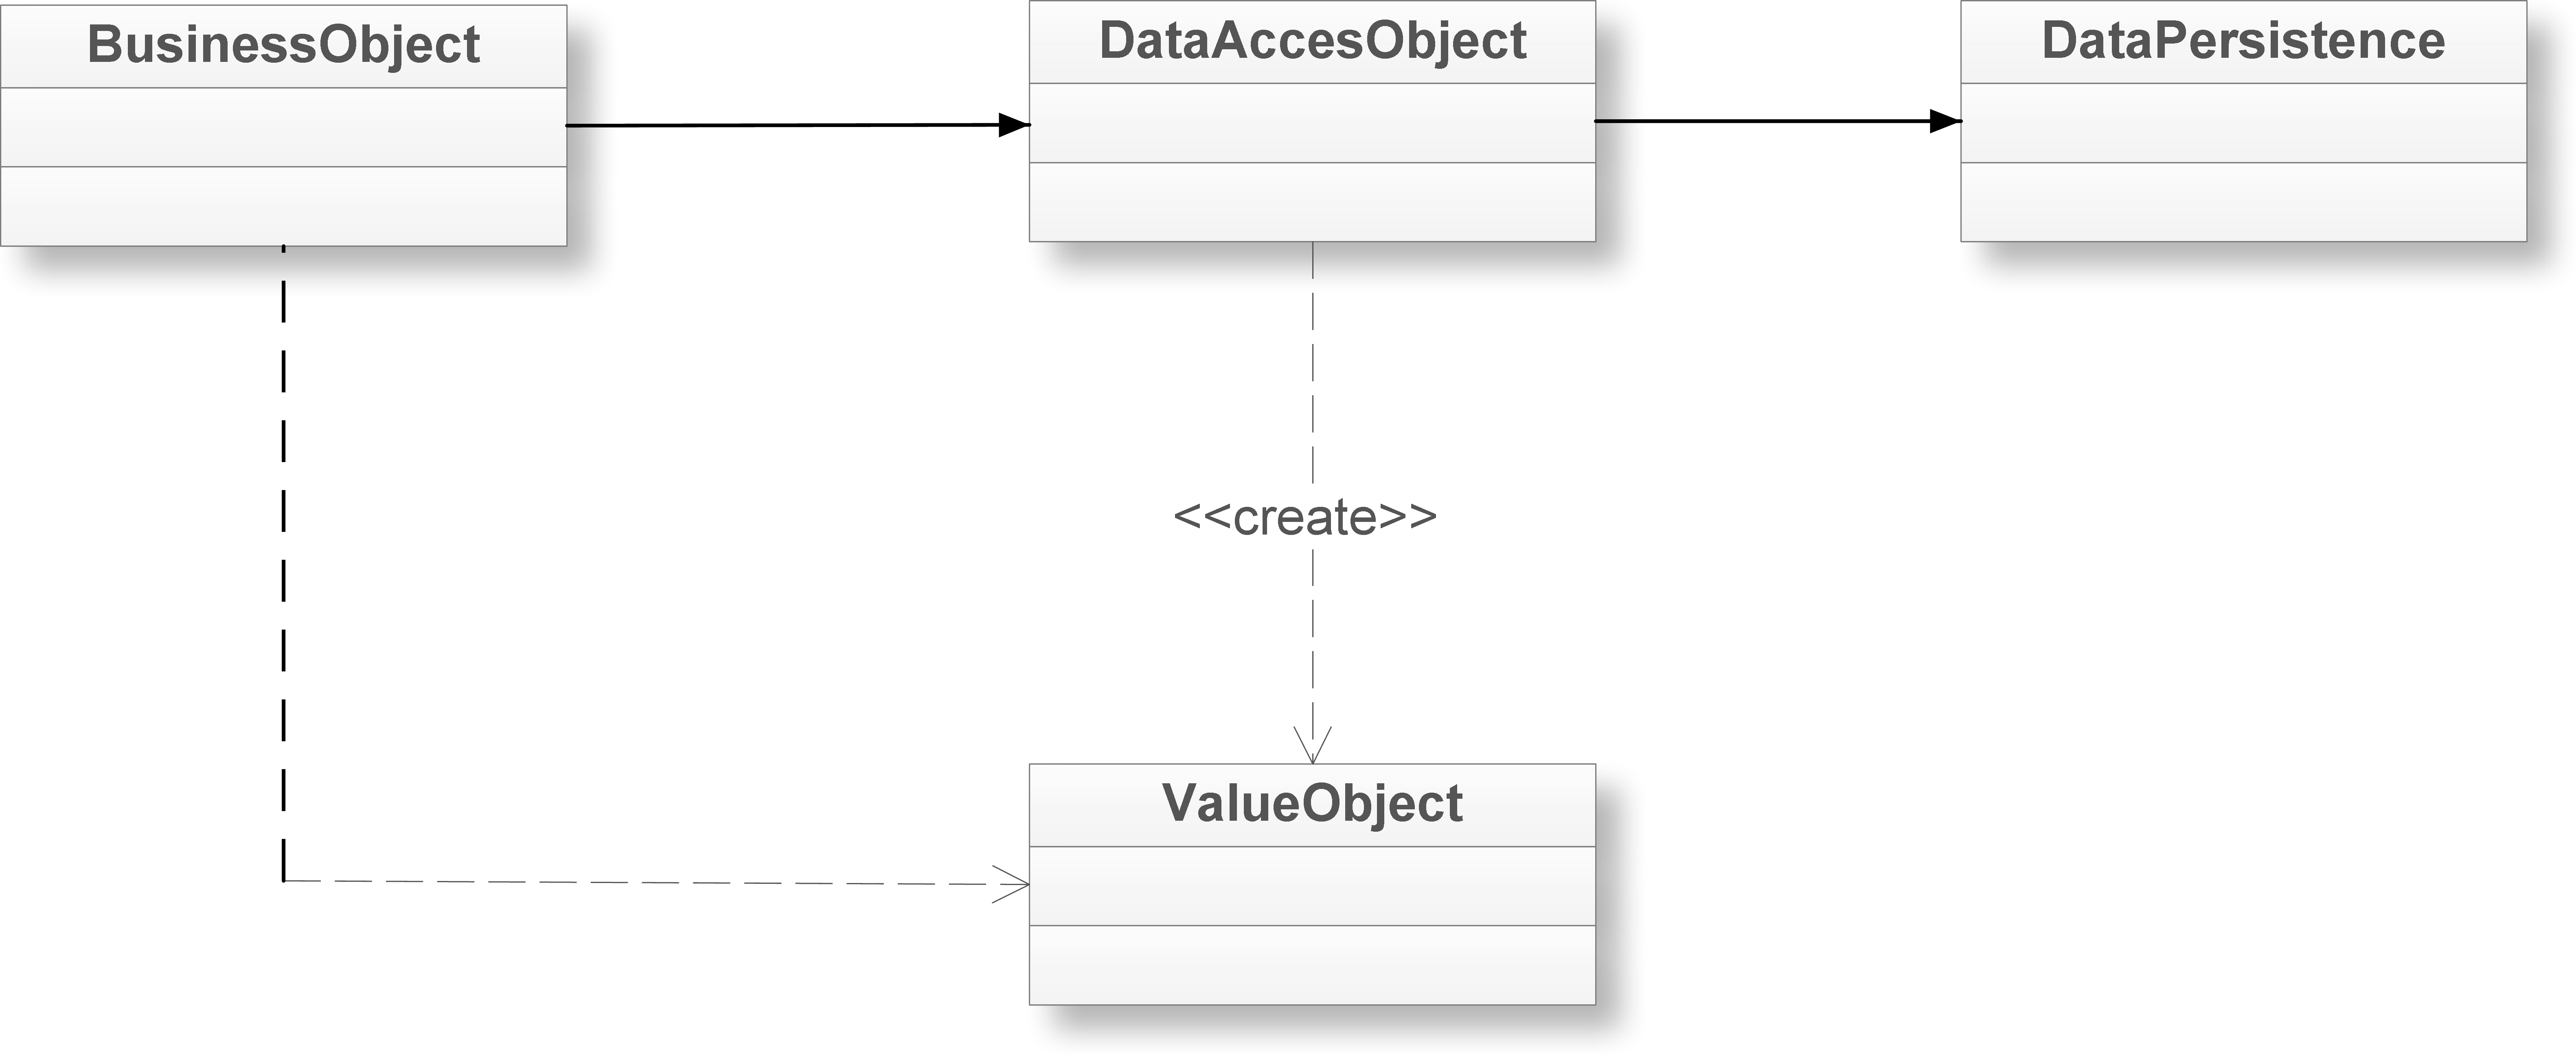
\includegraphics[width=.8\textwidth]{dao}
\caption{Diagramma ad alto livello del pattern DataAccessObject.}\label{fig:dao}
\end{figure}

\subsubsection{Componenti che lo implementano}
\begin{description}
\item{\scshape\bfseries Gestione Database}\\
Le classi DAO consentono di isolare l'accesso alle tabelle del database dalla parte di business logic facendo corrispondere alle invocazioni di metodo le opportune operazioni sui record del database.

L'utilizzo di tale pattern crea inoltre un maggiore livello di astrazione e mantiene una rigida separazione tra le sotto-architetture corrispondenti a model e presenter.
\end{description}

\subsection{Façade}

\subsubsection{Scopo}
Fornire un'interfaccia unificata per un insieme di interfacce o classi presenti in una sotto-architettura. Façade definisce inoltre un'interfaccia di livello più alto che rende la sotto-architettura più semplice da utilizzare.

\subsubsection{Diagramma esemplificativo}
\begin{figure}[h]
\centering
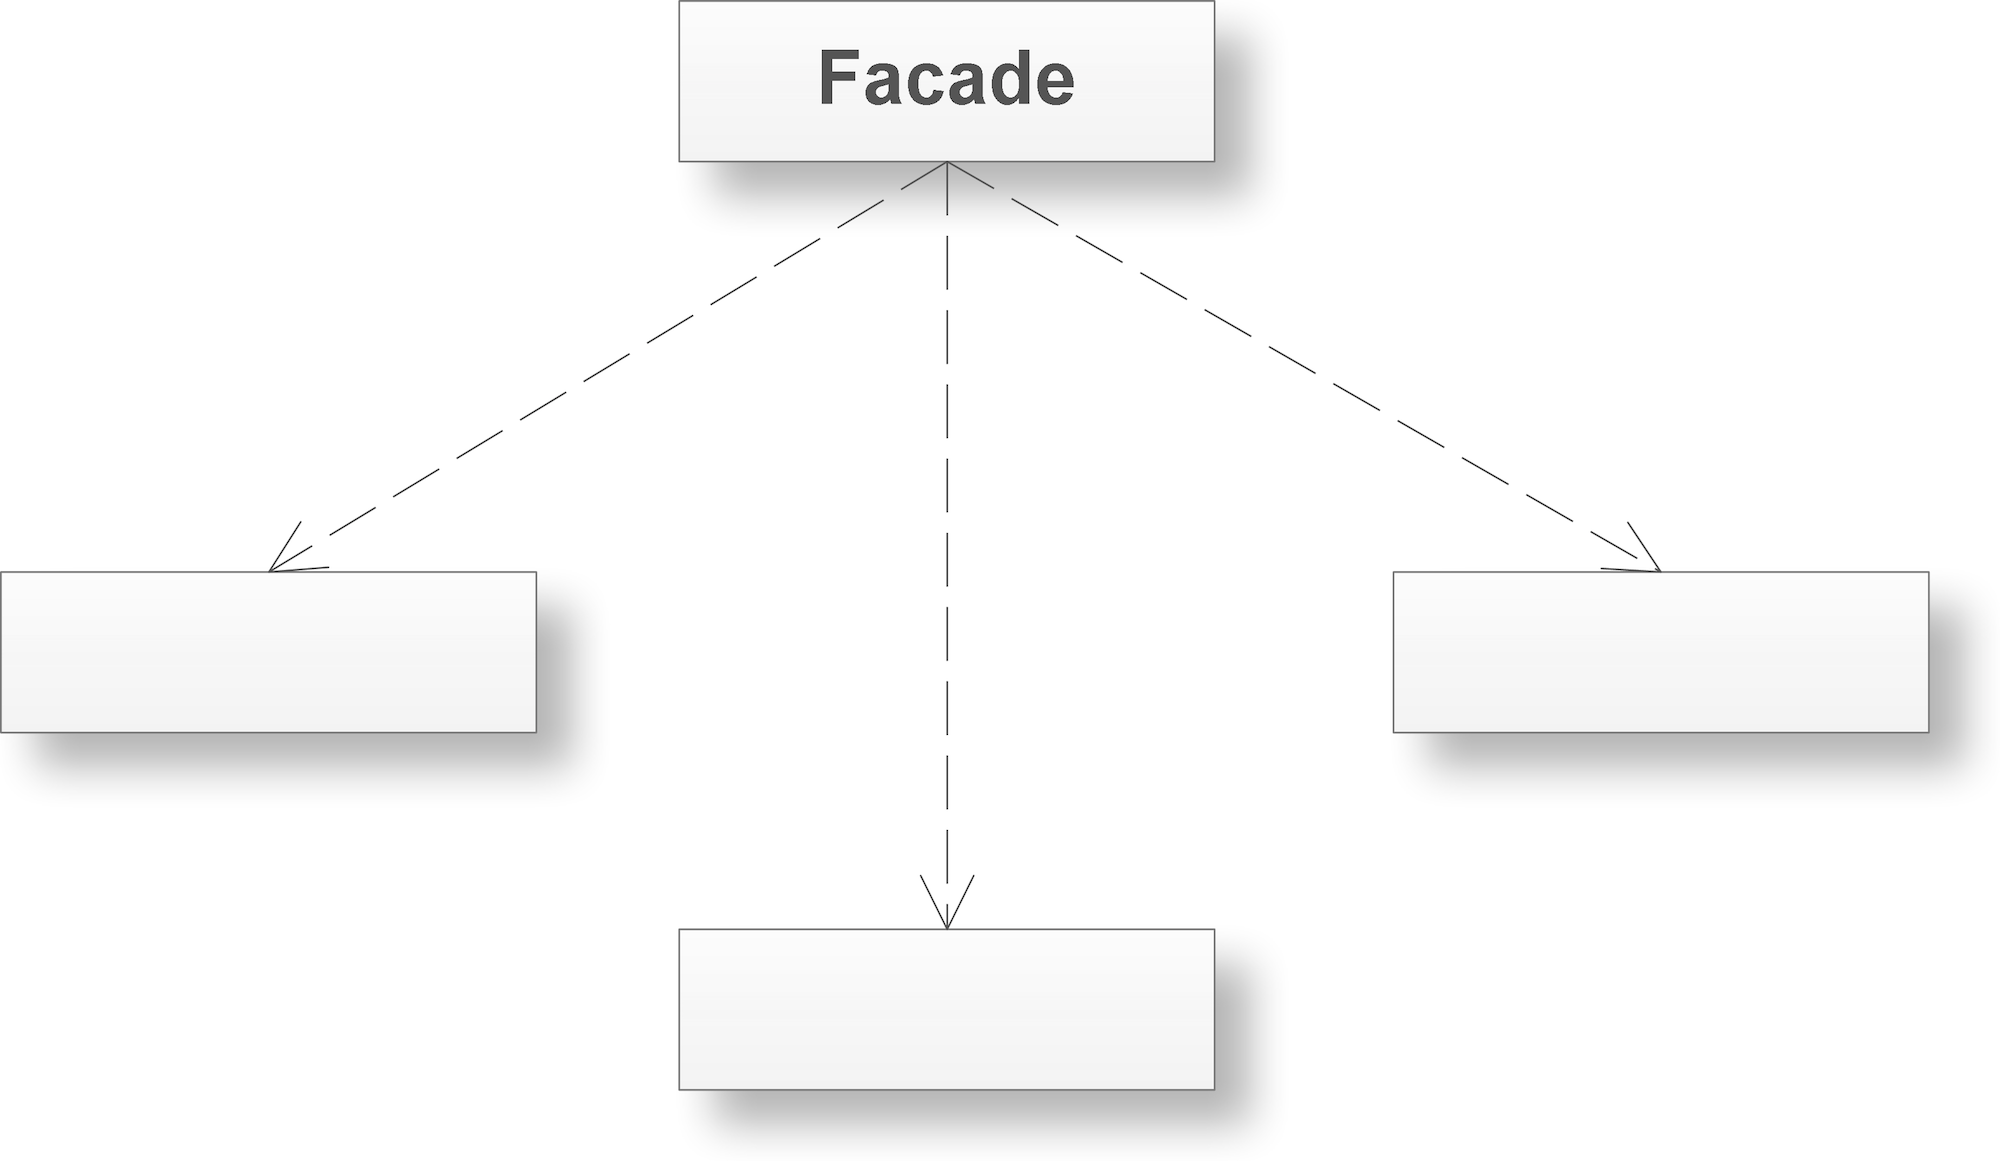
\includegraphics[width=.8\textwidth]{facade}
\caption{Diagramma ad alto livello del pattern Facade.}\label{fig:facade}
\end{figure}

\subsubsection{Componenti che lo implementano}
\begin{description}
  \item{\scshape\bfseries Façade del server}\\
L'uso di Façade permette di esporre verso i client una sorta di interfaccia semplificata nascondendo i componenti della sotto-architettura server, fornendo un punto di accesso centralizzato e riducendo il numero di dipendenze funzionali fra le classi del server e i componenti appartenenti a sotto-architetture esterne.
  \item{\scshape\bfseries Façade del presenter}\\
Tramite questo design pattern si introduce un livello di indirettezza fra le sotto-architetture clientpresenter e clientview, che risultano dunque indipendenti.
  \item{\scshape\bfseries Façade della vista}\\
Data la forte bidirezionalità delle interazioni fra componenti delle sotto-architettura clientpresenter e clientview, è stata introdotta una sorta di facciata anche alla vista in modo da facilitare il tracciamento delle dipendenze fra i componenti del presenter e quelli della view.
\end{description}

\subsection{Factory Method}

\subsubsection{Scopo}
Definisce un'interfaccia per la creazione di un oggetto, lasciando alle sottoclassi la decisione sulla classe concreta che deve essere istanziata e consente di deferire l'istanziazione di una classe alle sottoclassi.

\subsubsection{Diagramma esemplificativo}
\begin{figure}[h]
\centering
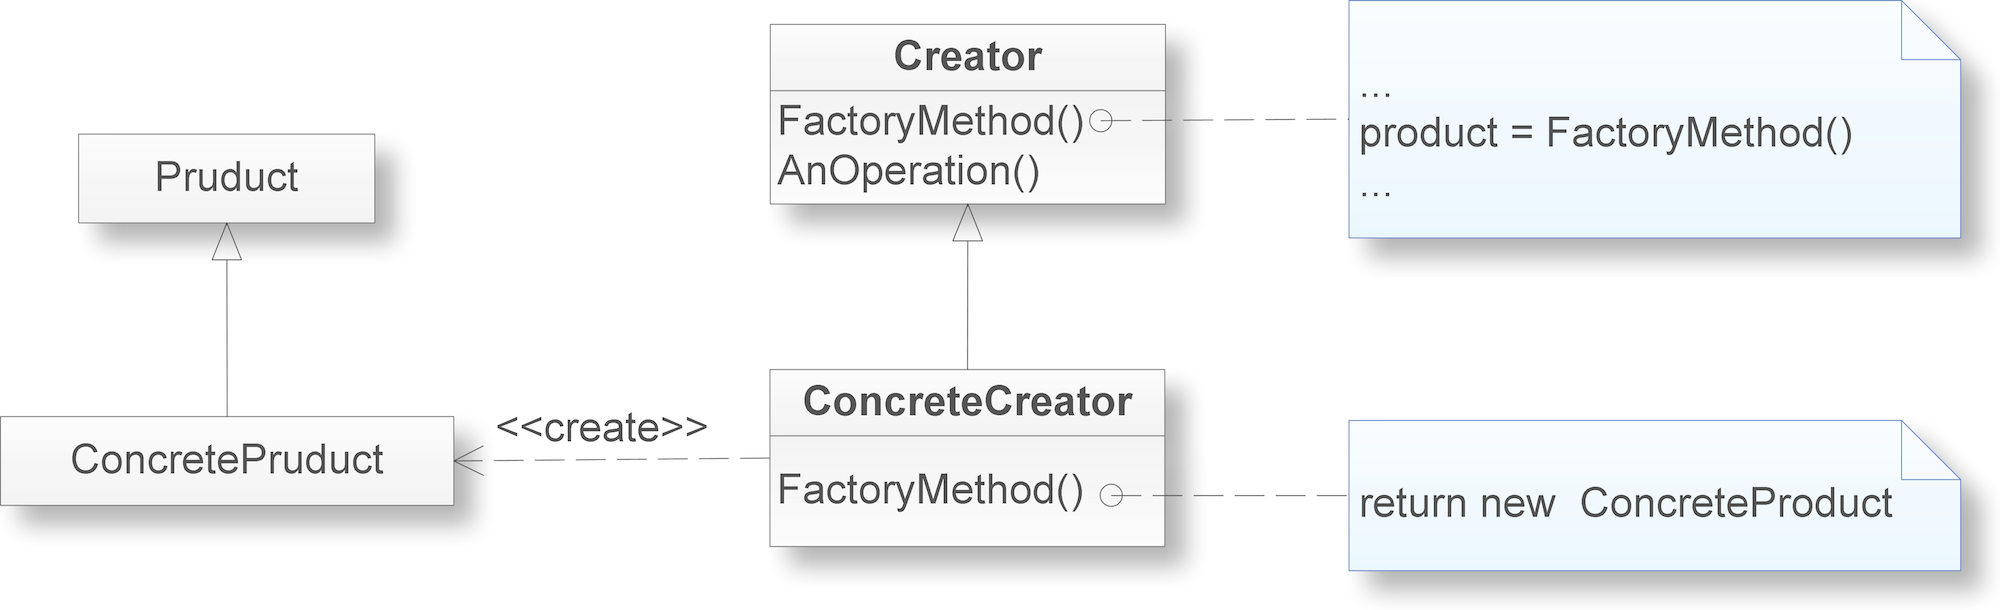
\includegraphics[width=.8\textwidth]{factory_method}
\caption{Diagramma ad alto livello del pattern Factory Method.}\label{fig:factory_method}
\end{figure}

\subsubsection{Componenti che lo implementano}
\begin{description}
  \item{\scshape\bfseries Facade del server}\\
Factory Method permette ai client di ottenere con facilità degli oggetti proxy che specializzano le interfacce \texttt{server.dao.IAudioMessage}, \texttt{server.dao.IAudioVideoMessage} e \texttt{server.dao.IUserData}.

Questo permette di ridurre il traffico di rete in quanto oggetti potenzialmente di grandi dimensioni rimangono sul server e vengono scaricati solo quando se ne presenta l'effettiva necessità.
  \item{\scshape\bfseries Gestione connessione}\\
Gli oggetti che rappresentano connessioni, sottotipi di \texttt{server.connection.IConnection} sono ottenuti mediante un Factory Method nelle classi concrete che implementano l'interfaccia \texttt{server.connectionICommunicationHandler}.

Ciò garantisce maggiore flessibilità in quanto permette in futuro di gestire più categorie di handler che restituiscono diversi tipi connessione.
\end{description}

\subsection{Model-View-Presenter}

\subsubsection{Scopo}
Il pattern architetturale \foreignlanguage{english}{Model-View-Presenter} similmente a quanto accade per \foreignlanguage{english}{Model-View-Controller} (MVC), ha lo scopo di mantenere separata la \textit{business logic}, cioè la gestione dei dati secondo le regole di un determinato dominio e la loro memorizzazione in forma persistente, dalla presentazione e manipolazione mediante interfaccia utente.

\subsubsection{Diagramma esemplificativo}
\begin{figure}[h]
\centering
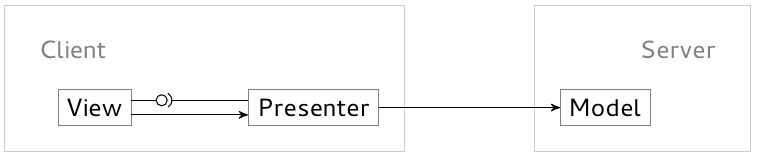
\includegraphics[width=.8\textwidth]{mvpHLdiagram}
\caption{Diagramma ad alto livello del pattern MVP.}\label{fig:mvpHL}
\end{figure}

\subsubsection{Componenti che lo implementano}
MVP viene utilizzato come il pattern più ad alto livello del nostro sistema. La distinzione fra model, presenter e view è infatti rispecchiata dalla suddivisione del sistema nelle tre sotto-architetture server, clientpresenter e clientview.

In generale, l'utilizzo di MVP riduce l'accoppiamento tra le sotto-architetture minimizzando le modifiche richieste a ognuno di essi come conseguenza di cambiamenti all'interno degli altri.

Inoltre, i componenti di questa sotto-architettura non sono vincolati a utilizzare la rete per accedere alle informazioni che sono memorizzate sul server quando queste sono già disponibili (e possono essere elaborate) sul client, migliorando quindi l'esperienza utente.

In particolare, le parti del sistema che usano questo pattern corrispondono alle sotto-architetture:
\begin{itemize}[noitemsep,nolistsep]
  \item server
  \item clientpresenter
  \item clientview}
\end{itemize}

\subsection{Observer}

\subsubsection{Scopo}
Definire una dipendenza uno a molti fra oggetti, in modo tale che se un oggetto cambia il suo stato tutti gli oggetti dipendenti da questo siano notificati e aggiornati automaticamente.

\subsubsection{Diagramma esemplificativo}
\begin{figure}[h]
\centering
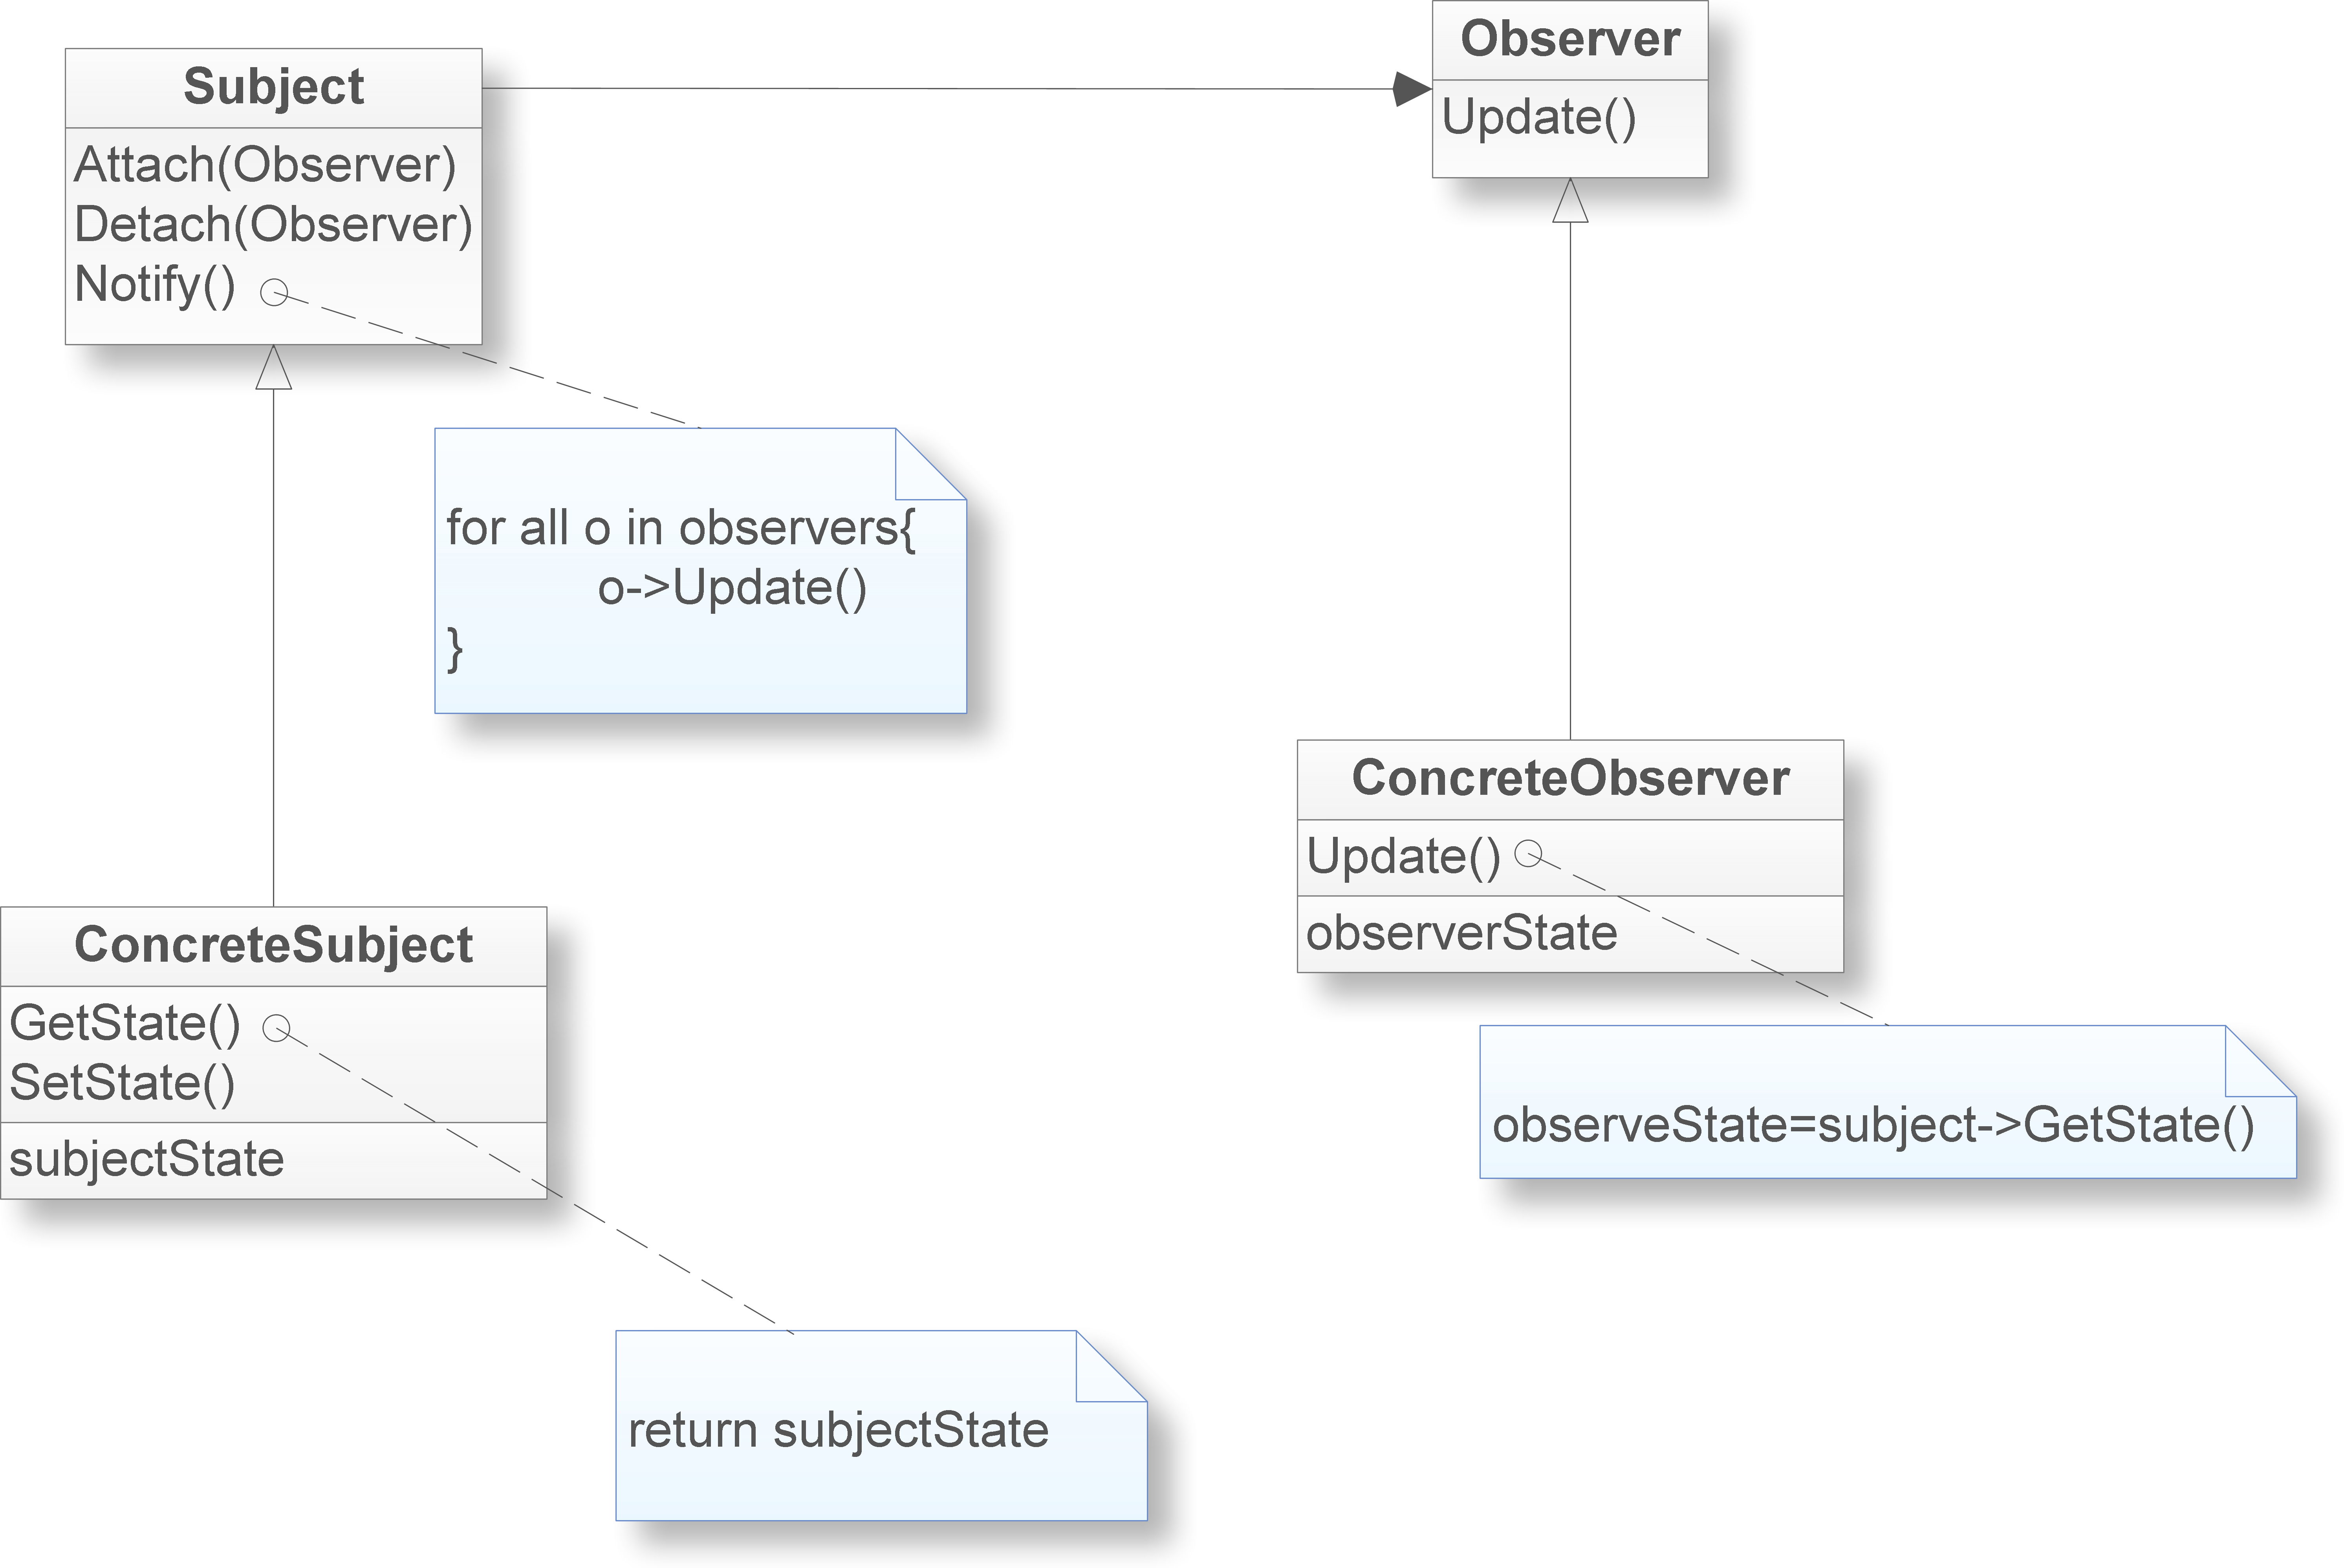
\includegraphics[width=.7\textwidth]{observer}
\caption{Diagramma ad alto livello del pattern Observer.}\label{fig:observer}
\end{figure}

\subsubsection{Componenti che lo implementano}
\begin{description}
  \item{\scshape\bfseries Gestione stato}\\
Il pattern Observer è utile in quanto permette agli utenti di osservare lo stato degli altri, ricevendo in modo automatico e trasparente una notifica nel caso in cui quest'ultimo subisse variazioni, essendo ogni utente sia osservato che osservatore.

Al momento della connessione, infatti, ogni utente si registra come osservatore sui suoi contatti che sono online e, al contempo, li aggiunge tra i propri osservatori. In tal modo gli utenti notificano in broadcast le loro variazioni di stato e sono sempre aggiornati sullo stato dei contatti della loro rubrica.
\end{description}

\subsection{Proxy}

\subsubsection{Scopo}
Fornisce un placeholder per un altro oggetto in modo da controllarne l'accesso e consentire un uso ottimizzato della memoria.

\subsubsection{Diagramma esemplificativo}
\begin{figure}
\centering
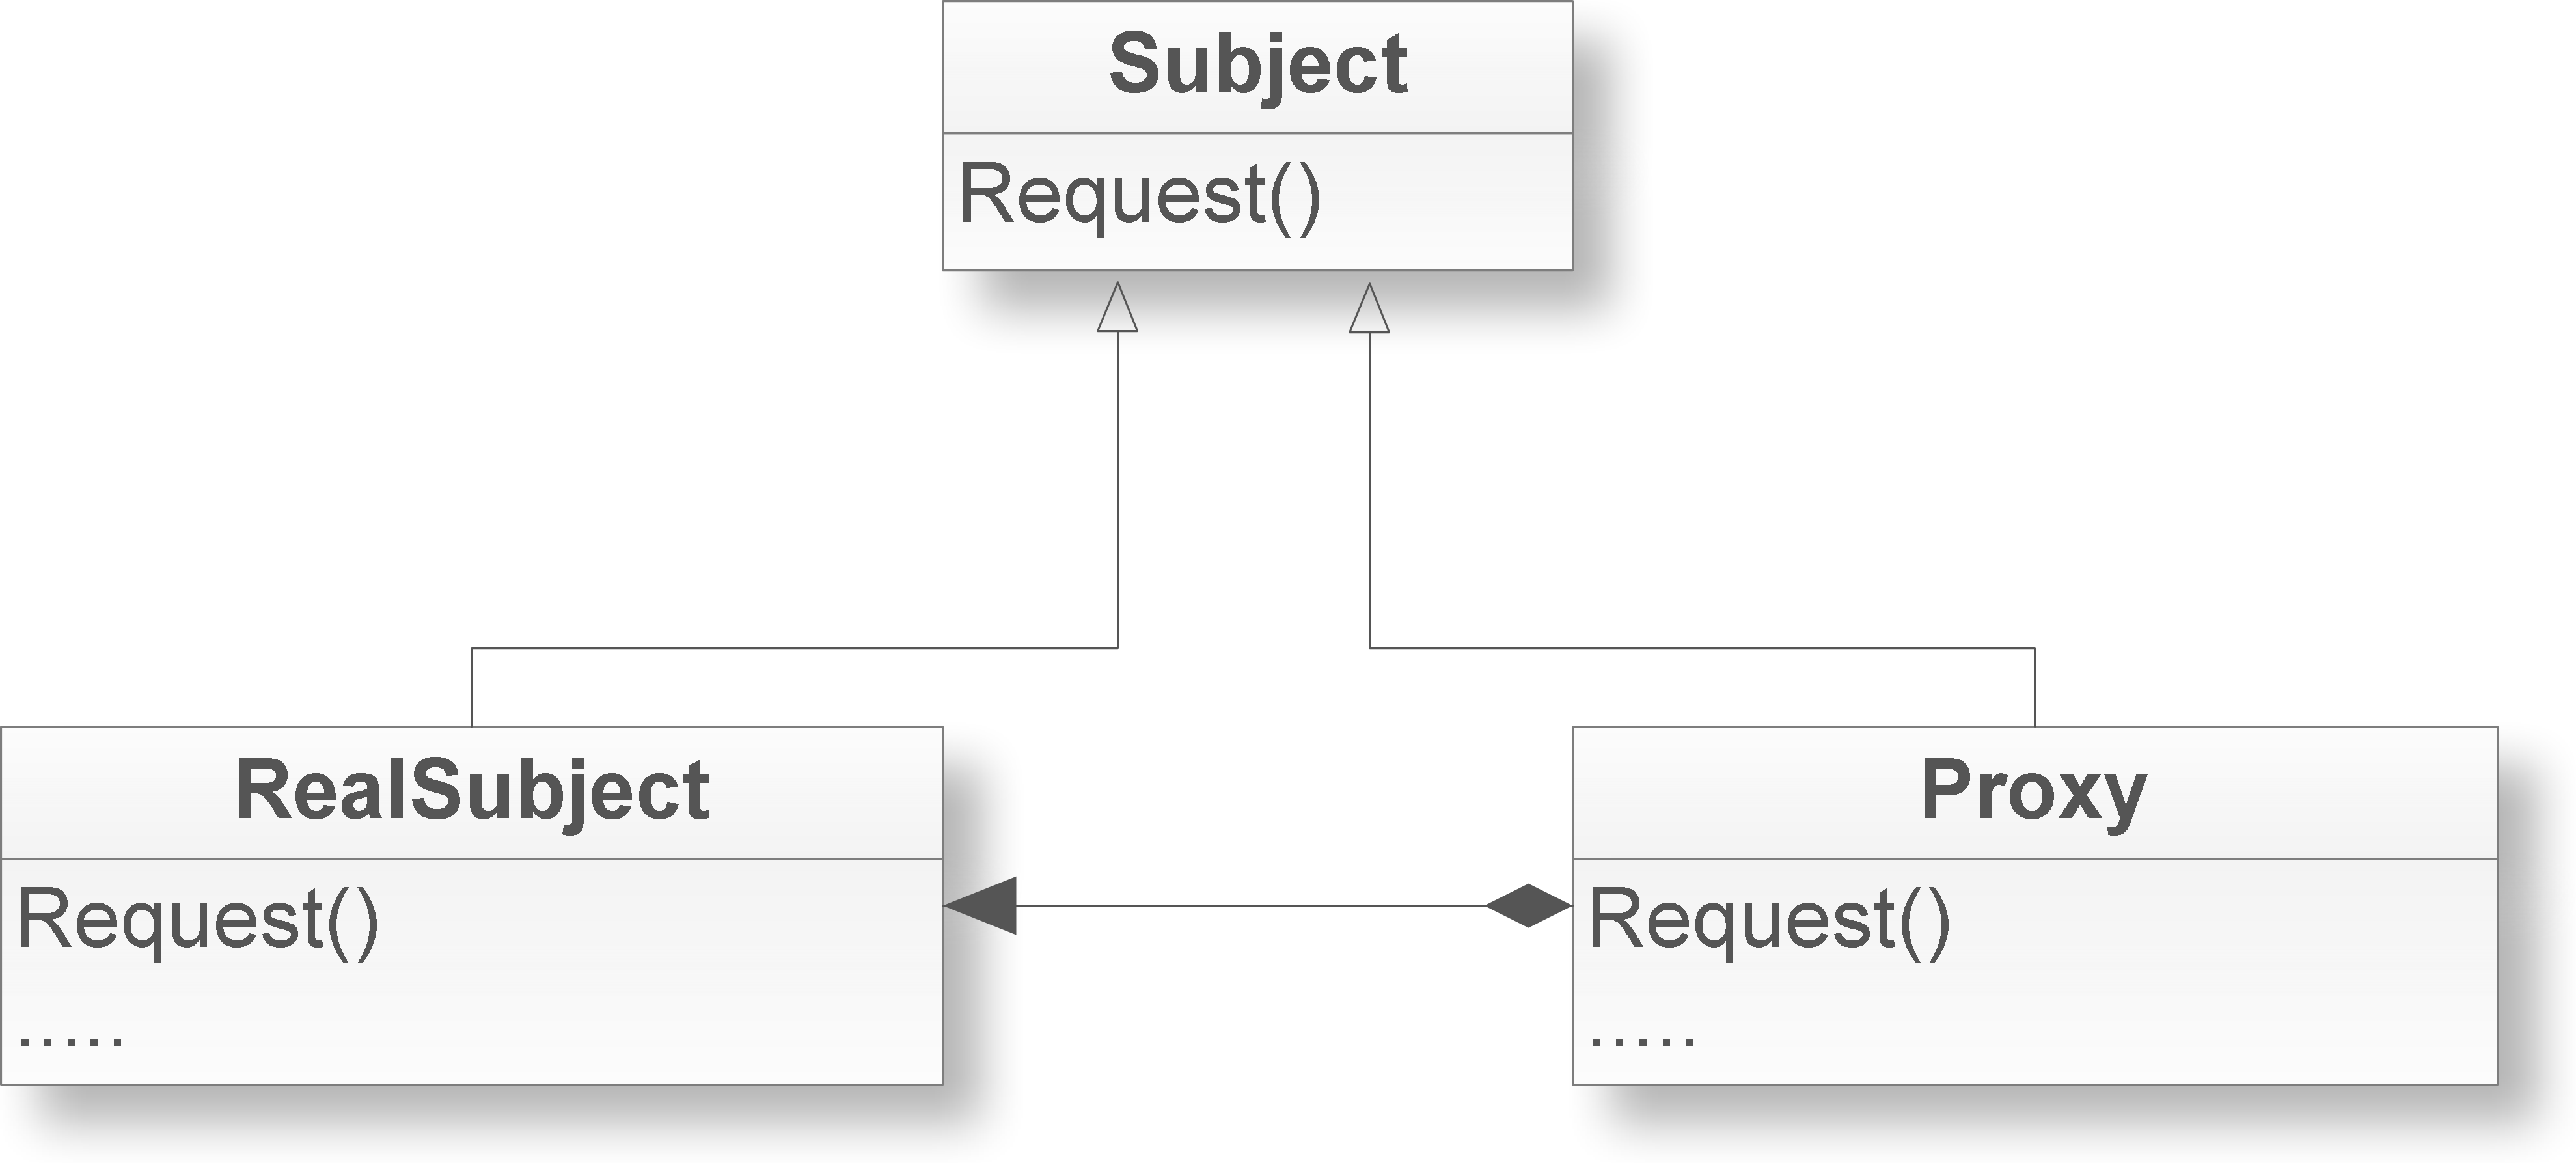
\includegraphics[width=.8\textwidth]{proxy}
\caption{Diagramma ad alto livello del pattern Proxy.}\label{fig:proxy}
\end{figure}

\subsubsection{Componenti che lo implementano}
\begin{description}
  \item{\bfseries\scshape Gestione rubrica}\\
L'utilizzo di un proxy al posto di un utente permette di raggiungere una maggiore efficienza limitando l'utilizzo della rete evitando all'utente di percepire una eccessiva lentezza che comprometterebbe la sua esperienza.

Inoltre, tramite un proxy è possibile controllare l'accesso ai dati (che risiedono nel server) garantendo dunque un migliore livello di protezione.
  \item{\bfseries\scshape Gestione segreteria}\\
Poiché i messaggi audio e, soprattutto, i messaggi audio/video possono essere di grandi dimensioni, i proxy permettono di ottimizzare il consumo della memoria e di evitare l'attesa da parte dell'utente se non strettamente necessario.
\end{description}

\subsection{Singleton}

\subsubsection{Scopo}
Il pattern creazionale Singleton, garantisce che una determinata classe possa essere istanziata una sola volta, e di fornirne un punto di accesso globale. Questo pattern va utilizzato negli ambiti in cui si ha la necessità che l'accesso ad una determinata entità sia unico, in modo da permettere la gestione ottimale della risorsa stessa.

\subsubsection{Diagramma esemplificativo}
\begin{figure}[h]
\centering
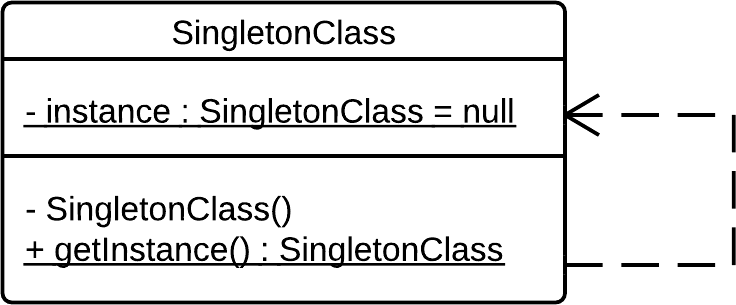
\includegraphics[width=.8\textwidth]{singleton}
\caption{Diagramma ad alto livello del pattern Singleton.}\label{fig:singleton}
\end{figure}

\subsubsection{Componenti che lo implementano}
\begin{description}
  \item{\scshape\bfseries Façade del server}\\
Il pattern Singleton pone un limite superiore stretto al numero di istanze che possono esistere di una determinata classe e perciò è utile utilizzarlo per poter controllare il numero di oggetti \texttt{server.StandardServerFacade} che in questo caso è pari a uno. L'unicità dell'oggetto façade garantisce la presenza di un solo punto di accesso alle funzionalità dell sotto-architettura server.
  \item{\scshape\bfseries Façade del presenter}\\
Il pattern Singleton è altresì utile per controllare il numero di istanze della classe \texttt{clientpresenter.StandardPresenterFacade} per gli stessi motivi evidenziati in precedenza, ossia l'unicità del punto di accesso alle funzionalità della sotto-architettura clientpresenter.
  \item{\scshape\bfseries Gestione connessione}\\
La classe \texttt{server.connection.StandardConnectionHandler} è implementata come Singleton in modo da centralizzare la responsabilità di creare nuove connessioni in risposta alle esigenze dei client.
\end{description}

\subsection{State}

\subsubsection{Scopo}
Permette ad un oggetto di cambiare il suo comportamento al variare del suo stato interno, quindi a run-time. L'oggetto si comporterà come se avesse cambiato la sua classe.

\subsubsection{Diagramma esemplificativo}
\begin{figure}[h]
\centering

\includegraphics[width=.7\textwidth]{state}
\caption{Diagramma ad alto livello del pattern State.}\label{fig:state}
\end{figure}

\subsubsection{Componenti che lo implementano}
\begin{description}
\item{Gestione dello Stato}\\
Il pattern State permette di gestire gli utenti del sistema determinando un comportamento diverso per questi ultimi a seconda del loro stato.

È stata definita un'apposita gerarchia di stati che permette quindi di specializzare nella maniera più adatta alle necessità del sistema le operazioni sugli utenti senza bisogno di condizionali annidati.
\end{description}
\clearpage

\section{Introduzione all'architettura di sistema}
Per introdurre l'architettura proposta è essenziale mettere in evidenza le seguenti considerazioni:
\begin{itemize}
	\item il sistema proposto dal team è dotato di una parte server ed una parte client;
	\item dopo un'analisi preliminare il team ha stabilito che la progettazione del server non deve essere vincolata da quella del client in modo tale da evitare che il progetto dell'applicativo lato server abbia la cognizione di come funziona il client. Ciò permetterà un futuro riutilizzo del codice (e.g. se si desiderasse creare un nuovo applicativo di tipo VOIP si potrà riutilizzare il server già creato);
	\item per quanto riguarda il lato client, al fine di garantire un alto livello di riutilizzo del codice e la possibilità di eseguire manutenzioni nel minor tempo possibile, si vuole che la logica d'implementazione del client sia svincolata dalla rappresentazione grafica del medesimo.
\end{itemize}

Tali considerazioni di base, hanno portato il team a suddividere l'architettura in tre sotto-architetture, intese anche come package:
\begin{itemize}
	\item il server (org.softwaresynthesis.mytalk.server);
	\item il clientpresenter (org.softwaresynthesis.mytalk.clientpresenter);
	\item il clientview (org.softwaresynthesis.mytalk.clientview).
\end{itemize}

Le specifiche di ogni sotto-architettura saranno definite in seguito, nelle relative sezioni.

Inoltre si fa presente che l'architettura generale, intesa come agglomerato delle tre sotto-architetture precedentemente elencate, fa uso del pattern MVP\@

Sotto tale ottica la sotto-architettura server ricopre il ruolo di model, il clientpresenter costituisce invece il presenter, mentre clientview è la vista definita per questo progetto. Tra le considerazioni più interessanti che hanno portato alla scelta di questo pattern, va messa in evidenza la seguente.

Assegnando ad ogni sotto-architettura un ruolo specifico, si garantisce un alto livello di riutilizzo del codice (e.g. clientview comunica con il presenter poiché non conosce la logica di business del sistema).

Quindi in un futuro di potrebbe riprendere la vista oggi definita, e riutilizzarla in un altro progetto, andando solo a ridefinire, se necessario, un presente che riproponga una nuovo adattamento della parte logica.

Di seguito verranno proposte le sotto-architetture evidenziate. Di ogni una sarà dato un elenco dettagliato dei componenti che lo interessano. Si sottolinea che per componenti non si intende i sottopackage, ma gli agglomerati di classi (potenzialmente prese da package diversi) che concorrono ad un fine comune: la definizione delle funzionalità del componente trattato.
\clearpage

\section{Architettura mytalk.server}
Tale sotto-architettura definisce le specifiche e le funzionalità dell'applicativo lato server. In esso saranno definiti i seguenti componenti:
\begin{itemize}[noitemsep,nolistsep]
	\item Gestione Database.
	\item Gestione connessione.
	\item Gestione rubrica.
	\item Gestione stato.
	\item Gestione segreteria.
	\item Façade del server.
\end{itemize}

I componenti sopracitati verranno definiti di seguito. Si sottolinea sin da ora che il server è l'unico in grado di comunicare con il database su cui regge l'applicativo.

Infine, si fa notare che i nomi di tutte le classi riportate nella sezione sono implicitamente parte del package \texttt{org.softwaresynthesis.mytalk.server} pertanto tale prefisso sarà omesso nella loro denominazione.

\subsection{Componenti evidenziati}

\subsubsection{Gestione database}
\begin{description}
\item{\scshape\bfseries Descrizione:}\\
Gestione Database è il componente che si occupa di rappresentare la struttura del database relazionale su cui poggia l'applicativo. Le singole classi in esso definite rappresentano quindi le tabelle del database. In termini tecnici le classi interne al componente Gestione database implementa il design pattern DAO\@.

Tramite questo componente, il sistema potrà quindi effettuare operazione di lettura e scrittura di entità all'interno del database. Le classi che costituiscono il componente dovranno quindi essere dotate di:

\begin{itemize}
	\item metodi get per restituire i singoli attributi dell'istanza;
	\item metodi set per garantire un corretto inserimento dei dati prima di registrare l'istanza nel database.
\end{itemize}

Si informa inoltre che le classi di tale componente dovranno interagire con il \underline{framework} Hibernate, al fine di ottenere lo scopo precisato.

	\item{\scshape\bfseries Diagramma delle classi:}
	%TODO inserire il diagramma delle classi
	
	\item{\scshape\bfseries Classi utilizzate:}
	\begin{itemize}[nolistsep, noitemsep]
	  \item[-] \texttt{dao.AudioMessage}
	  \item[-] \texttt{dao.AudioVideoMessage}
	  \item[-] \texttt{dao.IAudioMessage}
	  \item[-] \texttt{dao.IAudioVideoMessage}
	  \item[-] \texttt{dao.IGroup}
	  \item[-] \texttt{dao.IUserData}
	  \item[-] \texttt{dao.StandardGroup}
	  \item[-] \texttt{dao.StandardUserData}
	\end{itemize}
\end{description}

\subsubsection{Gestione connessione}
\begin{description}
	\item{\scshape\bfseries Descrizione:}\\
Tale componente ingloba le classi destinate a stabilire le routine di connessione. A tal fine è stata definita l'interfaccia di una classe Singleton \texttt{connection.ICommunicationHandler}, implementata da \texttt{connection.StandardCommunicationHandler} che ha il compito di creare oggetti connessione. Le specifiche di tali oggetti sono descritte dall'interfaccia \texttt{connection.IConnection}, con la relativa implementazione \texttt{connection.WebRTCInfo}.
	\item{\scshape\bfseries Diagramma delle classi:}
	%TODO inserire il diagramma delle classi del componente gestione connessione
	\item{\scshape\bfseries Classi utilizzate:}
	\begin{itemize}[nolistsep, noitemsep]
	  \item[-] \texttt{connection.ICommunicationHandler}
	  \item[-] \texttt{connection.StandardCommunicationHandler}
	  \item[-] \texttt{connection.IConnection}
	  \item[-] \texttt{connection.WebRTCInfo}
	\end{itemize}
\end{description}

\subsubsection{Gestione rubrica}
\begin{description}
	\item{\scshape\bfseries Descrizione:}\\
La rubrica è organizzata in gruppi e sono previste due categorie di default: la \textit{blacklist} e la \textit{whitelist}.

L'utente può aggiungere ulteriori gruppi in base alle sue esigenze ma esclusivamente all'interno della \textit{whitelist}. Per trattare in maniera omogenea i gruppi di contatti e i singoli contatti si è utilizzato il design pattern Composite.

In particolare, \texttt{abook.IContact} rappresenta l'interfaccia principale comune a ogni tipologia di contatto e viene estesa dalle due interfacce \texttt{dao.IUserData} e \texttt{dao.IGroup}.

Il componente comprende anche l'interfaccia \texttt{abook.IAddressBook} e la relativa implementazione \texttt{abook.AddressBook}. Nell'implementazione specificata \texttt{abook.Addressbook} vincola il sistema a garantire che ogni utente abbia i due gruppi di default sopra descritti, come richiesto dai requisiti.

Infine, la classe \texttt{abook.UserDataProxy} viene utilizzata come proxy per lo scambio di dati fra la sotto-architettura server e la sotto-architettura clientpresenter.
	\item{\scshape\bfseries Diagramma delle classi:}
	%TODO inserire il diagramma delle classi del componente gestione rubrica
	\item{\scshape\bfseries Classi utilizzate:}\\
	\begin{itemize}[nolistsep, noitemsep]
	  \item[-] \texttt{abook.AddressBook}
	  \item[-] \texttt{abook.IAddressBook}
	  \item[-] \texttt{abook.IContact}
	  \item[-] \texttt{abook.UserDataProxy}
	  \item[-] \texttt{dao.IGroup}
	  \item[-] \texttt{dao.IUserData}
	\end{itemize}
\end{description}

\subsubsection{Gestione stato}
\begin{description}
	\item{\scshape\bfseries Descrizione:}\\
Le classi di tale componente sono utilizzate per gestire lo stato degli utenti, permettendo un comportamento diverso delle istanze di \texttt{dao.StandardUserData} a seconda dello stato in cui si trova l'utente corrispondente. Gli stati possibili sono in prima istanza ``online'' e ``offline'', rappresentati dalle classi \texttt{state.StateOnline} e \texttt{state.StateOffline} rispettivamente.

Gli utenti che si trovano nello stato online possono trovarsi in due situazioni: ``occupato'' o ``disponibile'', rappresentati a loro volta dalle classi \texttt{state.StateOccupied} e \texttt{state.StateAvailable}.

Se l'utente è impegnato in una conversazione con uno o più utenti, allora lo stato in cui si trova è ``occupato''. Tuttavia, un utente può anche impostare manualmente il proprio stato ad ``occupato'' anche per segnalare di non essere disponibile a ricevere chiamate in ingresso.
	
La chiamata viene inoltre trattata in modo differente a seconda che l'utente si trovi nello stato ``disponibile'' o ``occupato''/``offline'', dal momento che nel primo caso la chiamata va a buon fine mentre nel secondo verrà attivato il meccanismo di segreteria telefonica.
	
Inoltre, i cambiamenti di stato vengono notificati a tutti gli utenti presenti in rubrica tali che si trovano nello stato online.
	\item{\scshape\bfseries Diagramma delle classi:}
	%TODO inserire il diagramma delle classi del componente gestione stato
	\item{\scshape\bfseries Classi utilizzate:}\\ 
	\begin{itemize}[noitemsep,nolistsep]
		\item[-] \texttt{dao.StandardUserData}
	    \item[-] \texttt{state.IState}
	    \item[-] \texttt{state.StateAvailable}
	    \item[-] \texttt{state.StateOccupied}
	    \item[-] \texttt{state.StateOffline}
	    \item[-] \texttt{state.StateOnline}
	\end{itemize}
\end{description}

\subsubsection{Gestione segreteria}
\begin{description}
	\item{\scshape\bfseries Descrizione:}\\
Il sistema di segreteria telefonica corrisponde all'interfaccia \texttt{message.IMessageBox} e alla relativa implementazione \texttt{message.StandardMessageBox} che permettono un accesso centralizzato all'insieme di messaggi che un determinato utente ha ricevuto.

I messaggi audio e audio/video sul server sono rappresentati dalle classi \texttt{dao.IAudioMessage} (implementata da \texttt{dao.AudioMessage}) e \texttt{dao.IAudioVideoMessage} (implementata da \texttt{dao.AudioVideoMessage}) rispettivamente.

L'onere di caricare in memoria e gestire l'interno contenuto del messaggio è posticipato al momento di effettiva necessità mediante l'utilizzo dei \textit{virtual proxy} corrispondenti alle classi \texttt{message.AudioMessageProxy} e \texttt{message.AudioVideoMessageProxy}.
	\item{\scshape\bfseries Diagramma delle classi:}
	%TODO inserire il diagramma delle classi del componente gestione rubrica
	\item{\scshape\bfseries Classi utilizzate:}
	\begin{itemize}[noitemsep,nolistsep]
	  \item[-] \texttt{dao.AudioMessage}
	  \item[-] \texttt{dao.AudioVideoMessage}
	  \item[-] \texttt{dao.IAudioMessage}
	  \item[-] \texttt{dao.IAudioVideoMessage}
	  \item[-] \texttt{message.AudioMessageProxy}
	  \item[-] \texttt{message.AudioVideoMessageProxy}
	\end{itemize}
\end{description}

\subsubsection{Façade del server}
\begin{description}
	\item{\scshape\bfseries Descrizione:}\\
L'interfaccia \texttt{IServerFacade} e la relativa implementazione \texttt{StandardServerFacade}, nella quale si è scelto di applicare il design pattern Singleton, forniscono una sorta di interfaccia alle funzionalità offerte dalla sotto-architettura server ai componenti che risiedono nel client.

Le funzionalità esposte consentono di gestire i messaggi presenti in segreteria, le richieste di comunicazione con altri utenti il login/registrazione degli utenti.
	\item{\scshape\bfseries Diagramma delle classi:}
	%TODO inserire il diagramma delle classi del componente façade del server
	\item{\scshape\bfseries Classi utilizzate:}\\
	\begin{itemize}[noitemsep,nolistsep]
	  \item[-] \texttt{IServerFacade}
	  \item[-] \texttt{StandardServerFacade}
	\end{itemize}
\end{description}

\subsection{Diagramma del package}
%TODO inserire il diagramma del package della sotto-architettura server

\subsection{Diagramma delle classi}
%TODO inserire il diagramma delle classi della sotto-architettura server
\clearpage

\section{Architettura mytalk.clientpresenter}
%TODO: da completare

Si fa notare che i nomi di tutte le classi riportate nella sezione sono implicitamente parte del package \texttt{org.softwaresynthesis.mytalk.clientpresenter} pertanto tale prefisso sarà omesso nella loro denominazione.

\subsection{Componenti evidenziati}

\subsubsection{Gestione comunicazione}
\begin{description}
	\item{\scshape\bfseries Descrizione:} 
		
	\item{\scshape\bfseries Diagramma delle classi:}
	\item{\scshape\bfseries Classi utilizzate:} 
	\begin{itemize}[noitemsep,nolistsep]
		\item[-] \texttt{IClient}
		\item[-] \texttt{StandardClient}
	\end{itemize}  
\end{description}

\subsubsection{Façade del presenter}
\begin{description}
	\item{\scshape\bfseries Descrizione:} 
Rappresenta l'interfaccia d'accesso verso la sotto-architettura clientpresenter. Tale componente svincola l'interfaccia grafica dal dover conoscere l'esatta sequenza di chiamata dei metodi per portare a conseguimento una determinata procedura.

%TODO poco chiara questa frase
I metodi del componente Façade del presenter hanno la cognizione dell'iter di chiamate a metodo per il corretto conseguimento della procedura. Il componente in esame richiede la definizione di un'interfaccia e una sua implementazione standard. Rimandiamo a tali classi per un approfondimento sul comportamento da seguire.
	\item{\scshape\bfseries Diagramma delle classi:}
	\item{\scshape\bfseries Classi utilizzate:} 
	\begin{itemize}[noitemsep,nolistsep]
		\item[-] \texttt{IPresenterFacade}
		\item[-] \texttt{StandardPresenterFacade}
	\end{itemize}
\end{description}

\subsection{Diagramma del package}
%TODO inserire diagramma di package del componente façade del presenter

\subsection{Diagramma delle classi}
%TODO inserire diagramma delle classi del componente façade del presenter
\clearpage

\section{Architettura mytalk.clientview}
%TODO da completare
Si fa notare che i nomi di tutte le classi riportate nella sezione sono implicitamente parte del package \texttt{org.softwaresynthesis.mytalk.clientview} pertanto tale prefisso sarà omesso nella loro denominazione.

\subsection{Componenti evidenziati}

\subsubsection{Façade della vista}
\begin{description}
	\item{\scshape\bfseries Descrizione:} 
%TODO da scrivere
	\item{\scshape\bfseries Diagramma delle classi:}
	%TODO inserire il diagramma delle classi del componente façade della vista
	\item{\scshape\bfseries Classi utilizzate:} 
	\begin{itemize}[noitemsep,nolistsep]
		\item[-] \texttt{boooooo}
	\end{itemize}  
\end{description}

\subsubsection{Gestione della GUI}
\begin{description}
	\item{\scshape\bfseries Descrizione:} 
%TODO da scrivere
	\item{\scshape\bfseries Diagramma delle classi:}
	%TODO inserire il diagramma delle classi del componente gestione della GUI
	\item{\scshape\bfseries Classi utilizzate:} 
	\begin{itemize}[noitemsep,nolistsep]
		\item[-] \texttt{boooooo}
	\end{itemize}  
\end{description}

\subsection{Diagramma del package}
%TODO inserire diagramma di package della sotto-architettura clientview

\subsection{Diagramma delle classi}
%TODO inserire diagramma delle classi della sotto-architettura clientview
\clearpage

\section{Descrizione delle classi}

\subsection{Package org.softwaresynthesis.mytalk.server.dao}

\subsubsection{IAudioMessage}
\begin{description}
	\item{\scshape\bfseries Descrizione:}\\
Interfaccia per i messaggi audio della segreteria telefonica che viene implementata dalle classi \texttt{AudioMessage} e dal suo proxy \texttt{message.AudioMessageProxy}.
% contiene operazione astratta play() per riprodurre il messaggio (se presente) o scaricarlo e avviarne la riproduzione
	\item{\scshape\bfseries Componenti che ne fanno uso:}
	  \begin{itemize}[noitemsep,nolistsep]
	  \item[-] Gestione database
	  \item[-] Gestione segreteria
	  \end{itemize}
\end{description}

\subsubsection{IAudioVideoMessage}
\begin{description}
	\item{\scshape\bfseries Descrizione:}\\
Interfaccia per i messaggi audio/video della segreteria telefonica, a sua volta implementata dalle classi \texttt{AudioVideoMessage} e dal relativo proxy \texttt{message.AudioVideoMessageProxy}.
% contiene operazione astratta play() per riprodurre il messaggio (se presente) o scaricarlo e avviarne la riproduzione
	\item{\scshape\bfseries Componenti che ne fanno uso:} 
	  \begin{itemize}[noitemsep,nolistsep]
	    \item[-] Gestione database
	    \item[-] Gestione segreteria
	  \end{itemize}
\end{description}

\subsubsection{AudioMessage}
\begin{description}
	\item{\scshape\bfseries Descrizione:}\\
Classe che rappresenta un messaggio audio nella segreteria telefonica di un utente, implementa l'interfaccia \texttt{IAudioMessage}.
	\item{\scshape\bfseries Componenti che ne fanno uso:}
	  \begin{itemize}[noitemsep,nolistsep]
	    \item[-] Gestione database
	    \item[-] Gestione segreteria
	  \end{itemize}
\end{description}

\subsubsection{AudioVideoMessage}
\begin{description}
	\item{\scshape\bfseries Descrizione:}\\
Classe che rappresenta un messaggio audio/video nella segreteria telefonica di un utente, implementa l'interfaccia \texttt{IAudioVideoMessage}.
	\item{\scshape\bfseries Componenti che ne fanno uso:}
	  \begin{itemize}[noitemsep,nolistsep]
	    \item[-] Gestione database
	    \item[-] Gestione segreteria
	  \end{itemize}
\end{description}

\subsubsection{IGroup}
\begin{description}
	\item{\scshape\bfseries Descrizione:}\\
Interfaccia per i gruppi interni alla rubrica, prevede un'operazione astratta \texttt{add(IUserData)} per l'aggiunta di un nuovo contatto al gruppo e un'operazione \texttt{remove(IUserData)} per la sua rimozione.

Estende inoltre l'interfaccia \texttt{abook.IContact} comune a tutti i contatti della rubrica e richiesta per l'applicazione del design pattern Composite.
	\item{\scshape\bfseries Componenti che ne fanno uso:} 
	  \begin{itemize}[noitemsep,nolistsep]
	    \item[-] Gestione database
	    \item[-] Gestione rubrica
	  \end{itemize}
\end{description}

\subsubsection{StandardGroup}
\begin{description}
	\item{\scshape\bfseries Descrizione:}\\
Implementazione dell'interfaccia \texttt{IGroup}, ogni gruppo è dotato di un nome e raccoglie in sé zero o più istanze di classi sottotipo di \texttt{abook.IContact}.
	\item{\scshape\bfseries Componenti che ne fanno uso:}
	  \begin{itemize}[noitemsep,nolistsep]
	    \item[-] Gestione database
	    \item[-] Gestione rubrica
	  \end{itemize}
\end{description}

\subsubsection{IUserData}
\begin{description}
	\item{\scshape\bfseries Descrizione:}\\
Interfaccia per le classi che rappresentano gli utenti, è dotata di operazioni get/set per accedere ai dati degli utenti registrati sul sistema.
	\item{\scshape\bfseries Componenti che ne fanno uso:}
	\begin{itemize}[noitemsep,nolistsep]
	  \item[-] Gestione database
	  \item[-] Gestione rubrica
	  \item[-] Gestione connessione
	\end{itemize}
\end{description}

\subsubsection{StandardUserData}
\begin{description}
	\item{\scshape\bfseries Descrizione:}\\
Classe che implementa l'interfaccia \texttt{dao.IUserData} le cui istanze corrispondono ai record della tabella degli utenti nel database.
	\item{\scshape\bfseries Componenti che ne fanno uso:}
	\begin{itemize}[noitemsep,nolistsep]
	  \item[-] Gestione database
	\end{itemize}
\end{description}

\subsection{Package org.softwaresynthesis.mytalk.server.connection}

\subsubsection{ICommunicationHandler}
\begin{description}
	\item{\scshape\bfseries Descrizione:}\\
Interfaccia per la gestione delle richieste per ottenere le informazioni necessarie a un client per stabilire una comunicazione con altri client. In particolare le operazioni in essa dichiarate dovranno ritornare un istanza di un oggetto che implementa \texttt{IConnection}.
	\item{\scshape\bfseries Componenti che ne fanno uso:}
		\begin{itemize}[noitemsep,nolistsep]
			\item[-] Gestione connessione
		\end{itemize}
\end{description}

\subsubsection{StandardCommunicationHandler}
\begin{description}
	\item{\scshape\bfseries Descrizione:}\\
La classe \texttt{StandardCommunicationHandler} è l'implementazione dell'interfaccia \texttt{ICommunicationHandler}. In tale classe, le informazioni ritornate al client sono informazioni necessarie a stabilire una connessione di tipo WebRTC (ritorna un istanza di \texttt{WebRTCInfo}).
	\item{\scshape\bfseries Componenti che ne fanno uso:}
		\begin{itemize}[noitemsep,nolistsep]
			\item[-] Gestione connessione
		\end{itemize}
\end{description}

\subsubsection{IConnection}
\begin{description}
	\item{\scshape\bfseries Descrizione:}\\
Interfaccia mediante la quale è possibile recuperare  i dati necessari a un client al fine di stabilire una connessione con un altro client.
	\item{\scshape\bfseries Componenti che ne fanno uso:}
		\begin{itemize}[noitemsep,nolistsep]
			\item[-] Gestione connessione
		\end{itemize}
\end{description}

\subsubsection{WebRTCInfo}
\begin{description}
	\item{\scshape\bfseries Descrizione:}\\
Implementazione dell'interfaccia \texttt{IConnection} che rappresenta le informazioni usate da un client per stabilire una connessione WebRTC con un altro client.
	\item{\scshape\bfseries Componenti che ne fanno uso:}
		\begin{itemize}[noitemsep,nolistsep]
			\item[-] Gestione connessione
		\end{itemize}
\end{description}

\subsection{Package org.softwaresynthesis.mytalk.server.abook}

\subsubsection{IContact}
\begin{description}
	\item{\scshape\bfseries Descrizione:}\\
Interfaccia condivisa da tutti i contatti della rubrica di un utente, permette di trattare in modo uniforme gli utenti singoli e i gruppi secondo quando previsto dal design pattern Composite.

Dichiara la presenza di operazioni astratte per recuperare l'accesso alle informazioni sottostanti (ad esempio il nome di un utente o di un gruppo).
	\item{\scshape\bfseries Componenti che ne fanno uso:}
	\begin{itemize}[nolistsep, noitemsep]
	  \item[-] Gestione rubrica
	  % forse gestione database
	\end{itemize}
\end{description}

\subsubsection{IAddressBook}
\begin{description}
	\item{\scshape\bfseries Descrizione:}\\
Interfaccia che raccoglie le operazioni sulla rubrica e permette di controllare l'accesso alle strutture dati che la implementano.
	\item{\scshape\bfseries Componenti che ne fanno uso:}
	\begin{itemize}[noitemsep,nolistsep]
	  \item[-] Gestione rubrica
	\end{itemize}
\end{description}

\subsubsection{UserDataProxy}
\begin{description}
  \item{\scshape\bfseries Descrizione:}\\
La classe implementa l'interfaccia \texttt{server.dao.IUserData} e rappresenta un proxy per i dati degli utenti che risiedono sul server.

Le istanze di questa classe vengono restituite da un opportuno Factory Method dichiarato nell'interfaccia \texttt{server.ServerFacade} e hanno il ruolo di rappresentare sui client degli oggetti che risiedono in un diverso spazio di indirizzamento (sul server) nonché di controllare gli accessi per esigenze di protezione.
  \item{\scshape\bfseries Componenti che ne fanno uso:}
  \begin{itemize}[noitemsep,nolistsep]
    \item[-] Gestione rubrica
  \end{itemize}
\end{description}

\subsubsection{AddressBook}
\begin{description}
	\item{\scshape\bfseries Descrizione:}\\
Classe che implementa l'interfaccia \texttt{IAddressBook} e rappresenta quindi la rubrica di un determinato utente. Contiene un riferimento a \texttt{IContact} che corrisponde al nodo padre della struttura dati ad albero contenente la rubrica.
	\item{\scshape\bfseries Componenti che ne fanno uso:}
	\begin{itemize}[noitemsep,nolistsep]
	  \item[-] Gestione rubrica
	\end{itemize}
\end{description}

\subsection{Package org.softwaresynthesis.mytalk.server.state}
\subsubsection{IState}
\begin{description}
	\item{\scshape\bfseries Descrizione:}\\
Interfaccia alla base della gerarchia di stati che gli utenti possono assumere nel corso dell'interazione con il sistema. La composizione delle istanze di \texttt{server.dao.StandardUserData} con oggetti sottotipo di \texttt{IState} cui inoltrano le richieste ricevute dall'esterno permette di cambiare dinamicamente il comportamento degli oggetti che rappresentano gli utenti.
	\item{\scshape\bfseries Componenti che ne fanno uso:}
	\begin{itemize}[noitemsep,nolistsep]
	  \item[-] Gestione stato
	  \item[-] Gestione connessione
	\end{itemize}
\end{description}

\subsubsection{StateOnline}
\begin{description}
	\item{\scshape\bfseries Descrizione:}\\
Classe astratta che implementa l'interfaccia \texttt{IState} e viene estesa da tutti gli stati che corrispondono alla presenza ``online'' dell'utente. È ulteriormente specializzata dalle sottoclassi concrete \texttt{StateAvailable} e \texttt{StateOccupied}, le quali hanno facoltà di determinare il reale comportamento degli utenti online.
	\item{\scshape\bfseries Componenti che ne fanno uso:}
	\begin{itemize}[noitemsep,nolistsep]
	  \item[-] Gestione stato
	\end{itemize}
\end{description}

\subsubsection{StateOffline}
\begin{description}
	\item{\scshape\bfseries Descrizione:}\\
Classe concreta della gerarchia degli stati che implementa l'interfaccia \texttt{IState} e corrisponde alla mancata presenza online dell'utente che la possiede. Un utente che si trova nello stato ``offline'' non può essere contattato direttamente ma solo attraverso la segreteria telefonica.
	\item{\scshape\bfseries Componenti che ne fanno uso:}
	\begin{itemize}[noitemsep,nolistsep]
	  \item[-] Gestione stato
	\end{itemize}
\end{description}

\subsubsection{StateAvailable}
\begin{description}
	\item{\scshape\bfseries Descrizione:}\\
Classe concreta della gerarchia degli stati che corrisponde alla presenza online di un utente e alla sua disponibilità ad accettare comunicazioni in ingresso.
	\item{\scshape\bfseries Componenti che ne fanno uso:}
    \begin{itemize}[noitemsep,nolistsep]
      \item[-] Gestione stato
    \end{itemize}
\end{description}

\subsubsection{StateOccupied}
\begin{description}
	\item{\scshape\bfseries Descrizione:}\\
Classe concreta della gerarchia degli stati che corrisponde alla mancata disponibilità di un utente a ricevere ulteriori comunicazioni in ingresso dal momento che si trova impegnato in un'altra conversazione. Gli utenti che si trovano in questo stato non possono essere contattati direttamente ma solo attraverso la possibilità di lasciare un messaggio in segreteria.
	\item{\scshape\bfseries Componenti che ne fanno uso:}
	\begin{itemize}[noitemsep,nolistsep]
	  \item[-] Gestione stato
	\end{itemize}
\end{description}

\subsection{Package org.softwaresynthesis.mytalk.server.message}
\subsubsection{IMessageBox}
\begin{description}
	\item{\scshape\bfseries Descrizione:}\\
Interfaccia che rappresenta, ad alto livello, la segreteria telefonica dell'utente cui è associata. Tramite opportune operazioni permette di accedere all'elenco dei messaggi audio o audio/video che l'utente ha ricevuto nel periodo in cui era in linea o non era disponibile perché impegnato in una conversazione.
	\item{\scshape\bfseries Componenti che ne fanno uso:}
	\begin{itemize}
	  \item[-] Gestione segreteria
	\end{itemize}
\end{description}

\subsubsection{StandardMessageBox}
\begin{description}
	\item{\scshape\bfseries Descrizione:}\\
Classe concreta che implementa l'interfaccia \texttt{IMessageBox} e rappresenta dunque la rubrica associata a un determinato utente.
	\item{\scshape\bfseries Componenti che ne fanno uso:}
	\begin{itemize}[noitemsep,nolistsep]
	  \item Gestione segreteria
	\end{itemize}
\end{description}

\subsubsection{AudioMessageProxy}
\begin{description}
	\item{\scshape\bfseries Descrizione:}\\
Proxy virtuale ad uso dei client per i messaggi audio lasciati ad un utente in segreteria. La classe implementa l'interfaccia \texttt{dao.IAudioMessage} ogni sua istanza è costruita per composizione con un riferimento a  \texttt{dao.AudioMessage}, cui inoltra le richieste dopo aver eventualmente scaricato il messaggio dal server.
	\item{\scshape\bfseries Componenti che ne fanno uso:}
	\begin{itemize}[noitemsep,nolistsep]
	  \item Gestione segreteria
	\end{itemize}
\end{description}

\subsubsection{AudioVideoMessageProxy}
\begin{description}
	\item{\scshape\bfseries Descrizione:}\\
Proxy virtuale ad uso dei client per i messaggi audio/video in segreteria. La classe implementa l'interfaccia \texttt{dao.AudioVideoMessage} ed è costruita, similmente a \texttt{AudioMessageProxy} con un'istanza di \texttt{dao.AudioVideoMessage} per limitare il traffico di rete e ottimizzare il consumo di memoria del client.
	\item{\scshape\bfseries Componenti che ne fanno uso:}
	\begin{itemize}[noitemsep,nolistsep]
	  \item Gestione segreteria
	\end{itemize}
\end{description}

\subsection{Package org.softwaresynthesis.mytalk.server}
\subsubsection{IServerFacade}
\begin{description}
	\item{\scshape\bfseries Descrizione:}\\
Interfaccia che contiene tutte le operazioni richieste dai componenti della sotto-architettura clientpresenter inerenti alla registrazione, all'autenticazione,  alla gestione della rubrica e della segreteria nonché delle connessioni con altri utenti.

In quest'ultimo caso, tuttavia, le operazioni richieste vengono a loro volta inoltrate al componente per la gestione della connessione (in particolare, verso \texttt{connection.IConnectionHandler}).
	\item{\scshape\bfseries Componenti che ne fanno uso:}
	\begin{itemize}[noitemsep,nolistsep]
	  \item[-] Façade del server
	  \item[-] Façade del presenter
	  \item[-] Gestione comunicazione
	\end{itemize}
\end{description}

\subsubsection{StandardServerFacade}
\begin{description}
	\item{\scshape\bfseries Descrizione:}\\
Questa classe Singleton è l'implementazione dell'interfaccia \texttt{IServerFacade} e contiene, in particolare, i metodi che rendono concrete le operazioni corrispondenti ai Factory Method dichiarati nell'interfaccia citata (per la gestione dei messaggi in segreteria e degli utenti nella rubrica).
	\item{\scshape\bfseries Componenti che ne fanno uso:}
	\begin{itemize}[noitemsep,nolistsep]
	  \item[-] Façade del server
	\end{itemize}
\end{description}

\subsection{Package org.softwaresynthesis.mytalk.clientpresenter}
\subsubsection{IClient}
%TODO da completare
\begin{description}
	\item{\scshape\bfseries Descrizione:}\\
	\item{\scshape\bfseries Componenti che ne fanno uso:} 
\end{description}

\subsubsection{StandardClient}
%TODO da completare
\begin{description}
	\item{\scshape\bfseries Descrizione:}\\
	\item{\scshape\bfseries Componenti che ne fanno uso:} 
\end{description}

\subsubsection{IPresenterFacade}
\begin{description}
	\item{\scshape\bfseries Descrizione:}\\
Interfaccia che raccoglie la dichiarazione di tutte le operazioni astratte con cui si suppone che la vista realizzi lo scambio di messaggi con il presenter. Tramite queste operazioni deve dunque essere possibile, ad esempio, gestire l'autenticazione di un utente, interrogare la segreteria telefonica, modificare lo stato e le informazioni personali e scaricare la rubrica.
	\item{\scshape\bfseries Componenti che ne fanno uso:}
	\begin{itemize}[noitemsep,nolistsep]
	  \item[-] Façade del presenter
	  %TODO anche le classi della sottoarchitettura clientview devono fare uso di questa interfaccia!
	\end{itemize}
\end{description}

\subsubsection{mytalk.client.StandardPresenterFacade}
\begin{description}
	\item{\scshape\bfseries Descrizione:}\\
Questa classe rappresenta un'applicazione del design pattern Singleton e implementa inoltre l'interfaccia \texttt{IPresenterFacade}. Fornisce pertanto dei metodi concreti utilizzati per la comunicazione fra la vista e il server, elaborando qualora necessario i dati ricevuti in input e inoltrando le richieste al componente Façade del server.
	\item{\scshape\bfseries Componenti che ne fanno uso:}
	\begin{itemize}[noitemsep,nolistsep]
	  \item[-] Façade del presenter
	\end{itemize}
\end{description}

\subsection{Package org.softwaresynthesis.mytalk.clientview}
%TODO mancano tutte le classi della sotto-architettura clientview
\clearpage

\section{Conclusioni sull'architettura}

\subsection{Diagrammi delle attività}

\subsection{Diagrammi di sequenza}
\clearpage

\section{Tracciamenti}
Nella seguente sezione vengono proposti tutti i tracciamenti eseguiti mediante il sistema Synthsis Requirment Manager. I tracciamenti proposti sono giustificati dalle seguenti due motivazioni:

\begin{itemize}
	\item Dimostrare il soddisfacimento per necessarietà e sufficienza della corrispondenza tra gli elementi tracciati (e.g. un componente deve rispondere necessariamente alle esigenze di uno o più requisiti, tali insomma che ne giustifichino l'esistenza. D'altro canto è richiesto che ogni requisito definito in fase d'analisi sia soddisfatto e risolto da almeno un componente).
	\item dare una lettura generale delle varie: componenti, requisiti, design pattern e classi.
\end{itemize}

\subsection{Tracciamenti Requisiti-Componenti}

\subsection{Tracciamenti Componenti-Requisiti}

\subsection{Tracciamenti Componenti-DesignPattern}

\subsection{Tracciamenti DesignPattern-Componenti}

\subsection{Tracciamenti Componenti-Classi}

\subsection{Tracciamenti Classi-Componenti}

\end{document}